% 相关版权与传播说明

% 本文档基于 MIT License 进行许可,部分内容参考来源:https://huanyushi.github.io/posts/labreport-template/ 和 https://www.yykspace.com/cn/index.html,非完全原创。

%!TEX program = xelatex
\documentclass[dvipsnames, svgnames, a4paper, 11pt]{article} 
% 指定文档类型为 article,使用 A4 纸张,字体大小为 11pt,并启用 dvipsnames 和 svgnames 颜色名称,以支持多种颜色的使用。

%---------------------------------------------------------------------
% 设定
%---------------------------------------------------------------------
\let\icon\liuyin  
\let\JMSection\ysySection
\let\JMRef\ysyRef
\let\JMEmph\ysyEmph
% ----------------------------------------------------- 
%	说明
% ----------------------------------------------------- 

% 本模板基于YSY的优秀实验报告模板进行优化,其完成了绝大部分工作,在此表示衷心感谢其支持与贡献。
% 无论您通过何种途径获得本文件,务必确保文件内容的隐私得到充分保护。请注意,本文件不支持上传任何平台,若因文件内容引发任何权益纠纷,文件的基础参与建设者将不承担任何责任。
% 若您愿意与我们进行进一步交流,欢迎通过以下网址与我们联系:https:// 。我们将在与相关人员沟通后,为您提供进一步的技术支持,我们相信通过基础的私信方式传播的文件一定程度上保证了您与我们的联系性。
% 若您通过某些途径获得此文件,希望你能成为遵守规则的人,祝您前程似锦,工作顺利,生活愉快!
% Jade Moon 与你同在!



% ----------------------------------------------------- 
%	设定
% ----------------------------------------------------- 


% ----------------------------------------------------- 
% 相较于最初的模板,我去掉了边框,去掉下面注释就能加回去。
%%	加边框的命令
%%	参考:https://tex.stackexchange.com/questions/531559/how-to-add-the-page-border-for-first-two-pages-in-latex
%\usepackage{tikz}
%\usetikzlibrary{calc}
%\usepackage{eso-pic}
%\AddToShipoutPictureBG{%
	%	\begin{tikzpicture}[overlay,remember picture]
		%		\draw[line width=0.6pt] % 边框粗细
		%		($ (current page.north west) + (0.6cm,-0.6cm) $)
		%		rectangle
		%		($ (current page.south east) + (-0.6cm,0.6cm) $); % 边框位置
		%\end{tikzpicture}}


% ----------------------------------------------------- 
% 自定义颜色
\usepackage{xcolor}
\definecolor{fblack}{HTML}{3E324A} % #3e324a(紫黑)
\definecolor{fgrayblue}{HTML}{5A6B84} % 灰蓝
\definecolor{fgraygreen}{HTML}{1C2F62} % #1c2f62 (物天)
\definecolor{fred}{HTML}{A52A2A} % 红蓝cp
\definecolor{fsilver}{HTML}{E6E4E0} % #e6e4e0(银白)
\definecolor{fbluegreen}{HTML}{BCC7D6} % 用于高亮
\definecolor{flameorange}{HTML}{D94352} % 红蓝cp


% ----------------------------------------------------- 
% 链接
\usepackage{ctex} % 字体
\usepackage[top=28mm,bottom=28mm,left=25mm,right=25mm]{geometry} % 最通用的边距设置:上下边距:28mm;左右边距:25mm
\usepackage{hyperref} 
\hypersetup{
	colorlinks,
	linktoc = section, % 超链接位置,选项有section, page, all
	linkcolor = fgrayblue, % linkcolor 目录颜色
	citecolor = fgrayblue,  % citecolor 引用颜色
	urlcolor = fgrayblue % 外部链接
}


% ----------------------------------------------------- 
% 引入必要的包
%A
\usepackage{amsmath,enumerate,multirow,float} % 1.提供增强的数学公式排版功能,如 align、gather 等环境。2.增强 enumerate 环境,允许指定编号格式。3.在表格中合并多行单元格。4.用于控制浮动体(如表格、图片)的放置,提供 H 选项让浮动体固定在当前位置。
\usepackage{tabularx} % 创建自动调整列宽的表格,比 tabular 更灵活。
\usepackage{fancyhdr} % 自定义页眉和页脚。
\usepackage{graphicx} % 插图
\usepackage{appendix} % 创建附录部分,允许 \appendix 轻松管理附录编号。
\usepackage{geometry}  % 页面调整
\usepackage{colortbl} % 给表格填充颜色
%B
\usepackage{lipsum} % 生成占位文本 \lipsum[1-3]。
\usepackage{adjustbox}% 调整表格大小
\usepackage{tabularray} % 绘制表格时可以更加方便添加框线
\usepackage{authblk} % 管理多作者信息。
\usepackage{wrapfig} % 让图片环绕文本。
\usepackage{subfig} % 创建多个子图。
%C
\usepackage{amsfonts} % 提供 \mathbb{}、\mathcal{} 等数学字体。
\usepackage{mathrsfs} % 提供花体数学字体,如 \mathscr{}。
\usepackage{calligra} % 提供书法风格字体,可用于 \textcalligra{}。
\usepackage{caption} % 自定义图片/表格标题格式。
\usepackage{physics} % 提供数学物理相关命令,如 \bra{}、\ket{}。
\usepackage{braket} % 提供 \braket{a|b} 量子力学符号。
\usepackage{amssymb} % 包含更多数学符号
\usepackage{amsmath} % 用于数学符号,特别是下标
\usepackage{booktabs} % 用于表格的好看线条


% ----------------------------------------------------- 
% 定义彩色环境
\usepackage{tcolorbox}
\tcbuselibrary{skins,breakable}

% 思考题
\newtcolorbox[auto counter,number within=section]{question}[1][]{
	breakable,
	enhanced, %跨页后不会显示下边框
	enhanced, breakable,
	%colback=fgrayblue!20!white,colframe=fgrayblue!80!black,colbacktitle = fgrayblue!80!black,
	colback=fgrayblue!20!white,colframe=fgrayblue,colbacktitle = fgrayblue, % 试试这个
	attach boxed title to top left = {yshift = -2mm, xshift = 5mm},
	boxed title style = {sharp corners},
	title={Reflection Question~\thetcbcounter:\quad},
	fonttitle=\bfseries,
	drop fuzzy shadow,
	#1
}

% 高亮
\newtcbox{\highlight}[1][fbluegreen]
{on line, arc = 0pt, outer arc = 0pt,
	colback = #1!85!white, colframe = white,
	boxsep = 0pt, left = 1pt, right = 1pt, top = 2pt, bottom = 2pt,
	boxrule = 0pt, bottomrule = 1pt, toprule = 1pt}

% 通用框架
\newtcolorbox{ubox}[2][]
{enhanced, breakable,
	colback = white, colframe = fbluegreen, coltitle = black,colbacktitle = fbluegreen,
	attach boxed title to top left = {yshift = -2mm, xshift = 5mm},
	boxed title style = {sharp corners},
	fonttitle = \bfseries,
	title={#2},#1}
	
% 代码块(仿MacOS的macbox)
\definecolor{wt1}{HTML}{ebebeb} % 白色主题的标题框顶部背景颜色
\definecolor{wt2}{HTML}{bebebe} % 白色主题的标题框底部背景颜色
\definecolor{wt3}{HTML}{efefef} % 白色主题的正文部分的背景颜色
\definecolor{circ1}{HTML}{eb605b} % 标题框左边第一个圆圈的颜色
\definecolor{circ2}{HTML}{f6bb31} % 标题框左边第二个圆圈的颜色
\definecolor{circ3}{HTML}{56cb45} % 标题框左边第三个圆圈的颜色
\definecolor{macosbox@bord}{RGB}{182,176,176}
\newtcolorbox{macbox}[2][]{
	enhanced,
	breakable,
	coltitle=black,
	colback = wt3,%macosbox@bg,
	boxrule=0mm,
	frame style={draw=macosbox@bord,fill=macosbox@bord},
	title style={top color=wt1,bottom color=wt2},
	drop fuzzy shadow=black,
	title={{\textcolor{circ1}{\huge$\bullet$}
			\textcolor{circ2}{\huge$\bullet$}
			\textcolor{circ3}{\huge$\bullet$}
			\hspace*{\fill}\texttt{#2}\hspace*{65mm}\hspace*{\fill}}},#1
}


% ---------------------------------------------------------------------
%	利用cleveref改变引用格式,\cref是引用命令
\usepackage{cleveref}
\crefformat{figure}{#2{\textcolor{fred}{\textbf{图 #1}}}#3} % 图片的引用格式
\crefformat{equation}{#2{(\textcolor{fred}{(#1)})}#3} % 公式的引用格式
\crefformat{table}{#2{\textcolor{fred}{\textbf{表 #1}}}#3} % 表格的引用格式
\crefformat{enumi}{#2{\textcolor{fred}{\textbf{[#1]}}}#3} % 文献的引用格式


% ---------------------------------------------------------------------
%	页眉页脚设置
\fancypagestyle{plain}{\pagestyle{fancy}}
\pagestyle{fancy}
\fancyhf{} % 清空默认页眉页脚
% 去掉页眉线(不想要页眉线把这行设为0pt,想要就改成这个\renewcommand{\headrule}{\color{fgraygreen}\hrule width\headwidth height 2pt})
\renewcommand{\headrulewidth}{0pt}
% 设置页脚线的颜色和粗细
\renewcommand{\footrule}{\color{fgraygreen}\hrule width\textwidth height 2pt}
% 自定义页眉
%\fancyhead[R]{\textcolor{fgrayblue}{电阻热噪声玻尔兹曼常量测量}}
% 自定义页脚内容
\fancyfoot[L]{\textcolor{fgrayblue}{黄罗琳,戴鹏辉,杨舒云,丁侯凯}}
\fancyfoot[R]{\textcolor{fgrayblue}{\textbf{\thepage}}}


% ---------------------------------------------------------------------
%	对目录、章节标题的设置
\renewcommand{\contentsname}{\centerline{\Huge 目录}}
\usepackage{titlesec}
\usepackage{titletoc}

% 【注意这里】由于学院logo实际上挺大的,有几百kb,所以你发现有点跑不动的话,你就把下面的section设置注释掉,换成这个
%\titleformat{\section}
%{\normalfont\bfseries\color{fgraygreen}\huge}
%{\thesection}
%{0.618}
%{}

% \titleformat{章节}[形状]{格式}{标题序号}{序号与标题间距}{标题前命令}[标题后命令]
\titleformat{\section}
{\normalfont\bfseries\color{fgraygreen}\huge}
{$\liuyin$}
{0.7em}
{}
\titleformat{\subsection}
{\normalfont\bfseries\color{fgrayblue}\LARGE} % 设置字体、大小、颜色
{\thesubsection} % 设置subsection编号的格式
{0.618em} % 编号和标题之间的间距
{}
\setcounter{secnumdepth}{3}
\titleformat{\subsubsection}
{\normalfont\bfseries\color{fgrayblue}\Large} 
{\thesubsubsection} 
{0.618em} 
{}


% ---------------------------------------------------------------------
% 图片、表格的设置(名称)
\captionsetup[figure]{labelfont={color=fgrayblue,bf},name=图} % 图片形式
\captionsetup[table]{labelfont={color=fgrayblue,bf},name=表} % 表格形式


% ---------------------------------------------------------------------
%   listing代码环境设置(不太好,将就用,有更好的可以自己改,其实一般也用不上)
\usepackage{listings}
\lstloadlanguages{python}
\lstdefinestyle{pythonstyle}{
	%backgroundcolor=\color{gray!6},% 用macbox就注释掉这一行
	language=python,
	frameround=tftt,
	%frame=shadowbox, % 用macbox就注释掉这一行
	keepspaces=true,
	breaklines,
	columns=spaceflexible,      
	basicstyle=\ttfamily\color{fblack}, % 基本文本设置(这里可以改改字号)
	keywordstyle=[1]\color{Yellow!75!black}\bfseries, 
	keywordstyle=[2]\color{flameorange!90!black},   
	stringstyle=\color{Purple!80!fblack},       
	showstringspaces=false,
	commentstyle=\ttfamily\color{Green!65!black},% 注释文本设置
	tabsize=2,
	morekeywords={as},
	morekeywords=[2]{np, plt, sp},
	numbers=left, % 代码行数
	numberstyle=\scriptsize\color{fgrayblue}, % 代码行数的数字字体设置
	stepnumber=1,
	numbersep=0pt % 代码行号和代码主体之间的距离,不用macbox就注释掉这一行
	%rulesepcolor=\color{fsilver} % 用macbox就注释掉这一行
}


% ---------------------------------------------------------------------
%	其他设置
\def\degree{${}^{\circ}$} % 角度
\graphicspath{{./images/}} % 插入图片的相对路径
\allowdisplaybreaks[4]  %允许公式跨页


% ---------------------------------------------------------------------
% 列表的设置
\usepackage{enumitem}
% 设置有序列表格式
\setlist[enumerate,1]{label=\textcolor{fblack}{\arabic*.}, font=\bfseries\color{fblack}}
\setlist[enumerate,2]{label=\textcolor{fblack}{(\arabic*)}, font=\bfseries\color{fblack}}
\setlist[enumerate,3]{label=\textcolor{fblack}{\roman*.}, font=\bfseries\color{fblack}}
\setlist[enumerate,4]{label=\textcolor{fblack}{(\roman*)}, font=\bfseries\color{fblack}}

%% 设置无序列表格式
\setlist[itemize,1]{label=\textcolor{fbluegreen}{$\blacktriangleright$}, font=\bfseries\color{fbluegreen}}
\setlist[itemize,2]{label=\textcolor{fbluegreen}{$\bullet$}, font=\bfseries\color{fbluegreen}}
\setlist[itemize,3]{label=\textcolor{fbluegreen}{$\blacksquare$}, font=\bfseries\color{fbluegreen}}

% 【注意这里】由于学院logo实际上挺大的,有几百kb,所以你发现有点跑不动的话,你就把下面的无序列表设置注释掉,换成上面那个
%\setlist[itemize,1]{label=$\liuyin$}
%\setlist[itemize,2]{label=\textcolor{fred}{$\blacktriangleright$}, font=\bfseries\color{fred}}
%\setlist[itemize,3]{label=\textcolor{fbluegreen}{$\bullet$}, font=\bfseries\color{fbluegreen}}


% ---------------------------------------------------------------------
% 封装
% 实验信息
\usepackage{ifthen}  
\newcommand{\infoTable}[9]{
    \begin{flushleft}
        \Huge \textcolor{fgraygreen}{\textbf{\kaishu #1}}  % 使用 ##1 来引用参数
    \end{flushleft}

    \vspace{-0.3cm}

    \begin{table}[h!]
        \textnormal{\textcolor{fgraygreen}{\rule{0.75\textwidth}{1.53pt} }}\\
        \begin{tabularx}{0.7\textwidth}{p{0.175\textwidth}p{0.525\textwidth}}
            \large\textcolor{fgraygreen}{\textbf{实验时间:}} &  \textbf{#2}\\
            \textcolor{fgraygreen}{\textbf{实验地点:}} &  \textbf{#3}\\
            \textcolor{fgraygreen}{\textbf{环境信息:}} &  \textbf{#4} \\
            \textcolor{fgraygreen}{\textbf{实验人1:}} &  \textbf{#5} \\
            \textcolor{fgraygreen}{\textbf{实验人2:}} &  \textbf{#6} \\
            \textcolor{fgraygreen}{\textbf{实验人3:}} &  \textbf{#7} \\
            \textcolor{fgraygreen}{\textbf{实验人4:}} &  \textbf{#8} \\
            \textcolor{fgraygreen}{\textbf{指导老师}} &  \textbf{#9}\\
        \end{tabularx}\\
        \textnormal{\textcolor{fgraygreen}{\rule{0.75\textwidth}{1.5pt} }}
    \end{table}
}

% 定义实验信息
\newcommand{\experimentNumber}[1]{\def\currentExperiment{#1}}  % 设置实验序号

% 定义页眉
\newcommand{\setExperimentHeader}{
    \ifthenelse{\equal{\currentExperiment}{E1}}{
        \fancyhead[R]{低温技术平台与高温超导研究} % 设置页眉为实验E1的名称
    }{
    \ifthenelse{\equal{\currentExperiment}{E2}}{
        \fancyhead[R]{ECDL外腔式半导体激光器实验} % 设置页眉为实验E2的名称
    }{
    \ifthenelse{\equal{\currentExperiment}{E3}}{
        \fancyhead[R]{光泵磁共振实验} % 设置页眉为实验E3的名称
    }{
    \ifthenelse{\equal{\currentExperiment}{E5}}{
        \fancyhead[R]{双光子纠缠源研究和量子非局域性验证实验} % 设置页眉为实验E5的名称
    }{
    \ifthenelse{\equal{\currentExperiment}{E6}}{
        \fancyhead[R]{散射光成像实验} % 设置页眉为实验E6的名称
    }{
        % 如果实验序号无效,则设置默认页眉
        \fancyhead[R]{实验未找到}
    }
    }}}}
}

% 定义生成实验信息表格的命令
\newcommand{\generateExperimentInfo}{
    \ifthenelse{\equal{\currentExperiment}{E1}}{
        % E1 实验信息
        \infoTable{E1: 低温技术平台与高温超导研究}
        {2025年3月21日、2025年3月28日}
        {教学楼物理实验室A101}
        {室温26\degree}
        {黄罗琳 22344001}
        {戴鹏辉 22344016} 
        {杨舒云 22344020} 
        {丁侯凯 22344009} 
        {王凯、章嘉伟}
    }{
    \ifthenelse{\equal{\currentExperiment}{E3}}{
        % E3 实验信息
        \infoTable{E3: 光泵磁共振实验}
        {2025年5月16日}
        {A407光学实验室}
        {室温25\degree}
        {黄罗琳 22344001}
        {戴鹏辉 22344016} 
        {杨舒云 22344020} 
        {丁侯凯 22344009} 
        {刘培亮}
    }{
    \ifthenelse{\equal{\currentExperiment}{E5}}{
        % E5 实验信息
        \infoTable{E5: 双光子纠缠源研究和量子非局域性验证实验}
        {2025年3月07日}
        {A102暗室}
        {室温24\degree}
        {黄罗琳 22344001}
        {戴鹏辉 22344016} 
        {杨舒云 22344020} 
        {丁侯凯 22344009} 
        {指导老师}
    }{
    \ifthenelse{\equal{\currentExperiment}{E6}}{
        % E6 实验信息
        \infoTable{E6: 散射光成像实验}
        {2025年5月30日}
        {A102}
        {室温23\degree}
        {黄罗琳 22344001}
        {戴鹏辉 22344016} 
        {杨舒云 22344020} 
        {丁侯凯 223440XX} 
        {指导老师}
    }
    }}}
}



% 定制的节
\newcommand{\JMSection}[1]{
	\section{#1}
	\vspace{-0.7cm} % 负值缩小间距
	\noindent\textcolor{fgraygreen}{\rule{0.382\textwidth}{2pt} }
	\vspace{7pt}
}

% 个人信息表(一人一表)
\newcommand{\infoPersonal}[6]{
	\renewcommand\arraystretch{1.4}
	\begin{tabularx}{\textwidth}{|X|X|X|X|}
		\hline
		专业: & #1 &年级: & #2\\
		\hline
		学生姓名: & #3 & 学号: & #4  \\
		\hline
		实验: & #5 & 日期: & #6\\
		\hline
	\end{tabularx}
}

% 粗糙的、用于偷懒的参考文献条目(中文版)
\newcommand{\JMRef}[7]{
	\item\label{ref:#1} #2\quad#3[#4]. \emph{#5}, #6, #7.
}

% 添加了学院配套主题图标
\newcommand{\liuyin}{\mathord{\raisebox{-0.2ex}{\includegraphics[height=0.8em]{images/theme/sysuspa_icon.png}}}}

% 强调
\newcommand{\JMEmph}[1]{
	\textbf{\textcolor{flameorange}{#1}}
}

% 加了一个评分表(来自原版)
\newcommand{\scoresTable}[8]{
	\begin{table}[h!]
		\renewcommand\arraystretch{1.7}
		\begin{tabularx}{\textwidth}{
				|X|X|X|X
				|X|X|X|X|}
			\hline
			\multicolumn{2}{|c|}{预习报告} & \multicolumn{2}{|c|}{实验记录} & \multicolumn{2}{|c|}{分析讨论} & \multicolumn{2}{|c|}{总成绩} \\
			\hline
			\centering#1&\centering#2 &\centering#3 &\centering#4 &\centering#5 &\centering#6 &\centering#7 &{\centering#8} \\
			\hline
		\end{tabularx}
	\end{table}
}


% ----------------------------------------------------- 
%	下面不用看,致敬原本的流萤主题
% ----------------------------------------------------- 


% ----------------------------------------------------- 
% 我还是不太能理解,为什么他们说今晚月色很美是含蓄的表白。 
% 直到我看到朝阳下江水漾起的片片金鳞、漆黑的夜空中不甘散去的橘黄云彩、亦或者是夜宵摊子上高谈阔论掺杂着串子被炭火炙烤出油香的烟火气息,都下意识拿出手机想跟你分享。 
% 我想把自己觉得美丽的东西传递给你。 
% 今天依然天晴,我亲爱的流萤。 
%---------------------------------------------------------------------
% 正文
%---------------------------------------------------------------------

\begin{document}
\experimentNumber{E6} 
\setExperimentHeader%自动生成页眉修改,自定义则如下所示
% 自定义页眉
%\fancyhead[R]{\textcolor{fgrayblue}{电阻热噪声玻尔兹曼常量测量}}
% 自定义页脚内容
%\fancyfoot[L]{\textcolor{fgrayblue}{黄罗琳,戴鹏辉,杨舒云,丁侯凯}}
%\fancyfoot[R]{\textcolor{fgrayblue}{\textbf{\thepage}}}


%给出当前实验组序号
% 实验信息列表:
% E1: 低温技术平台与高温超导研究
% E2: ECDL外腔式半导体激光器实验
% E3: 光泵磁共振实验
% E4: 晶体声光电光磁光实验
% E5: 双光子纠缠源研究和量子非局域性验证实验
% E6: 散射光成像实验
% E9: 自主研发光泵磁共振实验
% E10: 光纤特性研究与应用


% 实验报告主体部分,包含封面、前言、预习报告、实验主体内容以及附录。

    % 封面(主要修改实验参与人员和封面插图)
    % !TEX root = ../main.tex

\begin{titlepage}
	\newgeometry{margin = 0in}
	\parindent=0pt
	
	\hspace*{\fill} % 不用学院Logo就把这行注释掉
	
	\vspace{2em} % 不用学院Logo就把这行注释掉
	
	% 插图
	\begin{figure}[h!]
		\centering
		\includegraphics[width=0.8\linewidth]{images/theme/sysuspa_title}
	\end{figure}
	
	% 可选项(也就是不用学院logo,记得改注释)
%	\begin{figure}
%		\centering
%		\includegraphics[width=0.8\linewidth]{images/theme/snow_mountain_starry sky_aurora_2MB_cut}
%	\end{figure}
	
	\vspace{5em} % 不用学院Logo就把这行注释掉
	
	\begin{flushright}
		% 标题
		{ \Huge \bfseries 近代物理实验II实验报告} \hspace*{6em} \\[0.2cm]
		\rule{0.618\textwidth}{5pt} \hspace*{6em} \\[0.4cm]
		
		% 作者
		\LARGE\emph{\textbf{黄罗琳\quad 戴鹏辉\quad 杨舒云\quad 丁侯凯}} \hspace*{4.1em}	\\[0.7cm]
		
		% 地址
		\large\textbf{中山大学物理与天文学院,中国珠海市大学路 2 号,519082} \hspace*{5em}
		
	\end{flushright}
	
	% Bottom of the page
	\begin{center}
		\vfill
		
		% \Large\texttt{\textcolor{fgrayblue}{Zu messen heißt zu fragen, zu beobachten heißt zu lauschen, zu verstehen heißt zu enthüllen.}}
		%\Large\texttt{\textcolor{fgrayblue}{\kaishu 今古诸事,激荡中流,宏图待看新秀。}} % 试试这个,其实上面那个更高级
		\Large\texttt{\textcolor{fgrayblue}{\kaishu 珍重!}} % 试试这个,其实上面那个更高级
		
		\hspace*{\fill}
		
		{\LARGE \today}
		
		\hspace*{\fill}
	\end{center}
	
\end{titlepage}
    
    % 前言(填写实验基本信息)
    % !TEX root = ../main.tex

% 封面


%---------------------------------------------------------------------
% 评分栏
\begin{table}
	\renewcommand\arraystretch{1.7}
	\begin{tabularx}{\textwidth}{
			|X|X|X|X
			|X|X|X|X|}
		\hline
		\multicolumn{2}{|c|}{Preview Report}&\multicolumn{2}{|c|}{Experimental Record}&\multicolumn{2}{|c|}{Analysis \& Discussion}&\multicolumn{2}{|c|}{\Large\textbf{Total}}\\
		\hline
		\LARGE & & \LARGE & & \LARGE & & \LARGE & \\
		\hline
	\end{tabularx}
\end{table}


%---------------------------------------------------------------------
% 信息栏
\begin{table}
	\renewcommand\arraystretch{1.7}
	\begin{tabularx}{\textwidth}{|X|X|X|X|}
		\hline
		Grade \& Major: & 2022, Physics &Group number: & A2\\
		\hline
		Student name: & 杨舒云 \& 戴鹏辉  & Student number: & 22344020 \& 22344016\\
		\hline
		Experiment time: & 2024/9/25 & Teacher's Signature: & \\
		\hline
	\end{tabularx}
\end{table}


%---------------------------------------------------------------------
% 大标题
\begin{center}
	\huge \textbf{ET2-1 \quad 蓝牙音箱的焊接和调试\\Welding and Debugging of Bluetooth Speakers}
\end{center}


%---------------------------------------------------------------------
% 注意事项
\textbf{【Precautions】}
\begin{enumerate}
	\item The lab report consists of three parts:
	\begin{enumerate}
		\item \textbf{Prview Report}: Carefully study the experimental manual before class to understand the experimental principles; familiarize yourself with the instruments, equipment, and tools needed for the experiment, and their usage; complete the pre-lab thought questions; understand the physical quantities to be measured during the experiment, and prepare the experimental record forms in advance as required (you may refer to the experiment report template and print it if needed).
		\item \textbf{Experimental Records}: Meticulously and objectively record the experimental conditions, phenomena observed during the experiment, and data collected. Experimental records should be written in ballpoint pen or fountain pen and signed (\textcolor{fred}{\textbf{Records written in pencil are considered invalid}}). \textcolor{fred}{\textbf{Keep original records, including any errors and deletions; if a correction is necessary due to an error, it must be made according to the standard procedure.}} (Records should not be entered into a computer and printed, but handwritten notes can be scanned and printed); before leaving, have the experimental teacher check and sign the records. 
		\item \textbf{Data Processing and Analysis}: Process the raw experimental data (except for experiments that focus on learning the use of instruments), analyze the reliability and reasonableness of the data; present the data and results in a standardized manner (charts and tables), including numbering and referencing the data, charts, and tables sequentially; analyze the physical phenomena (including answering the experimental thought questions, writing out the thought process, and citing data as needed according to standards); finally, draw a conclusion.
	\end{enumerate}
	\textbf{The experiment report combines the preparation report, experimental records, and data processing and analysis, along with this cover page.}
	\item Submit the \textbf{experiment report} within one week after completing each experiment (under special circumstances, no later than two weeks).
\end{enumerate}


%---------------------------------------------------------------------
% 实验安全	
%\textbf{【Safety】}	
%\begin{enumerate}
%	\item 
%\end{enumerate}	
	
	
%---------------------------------------------------------------------	
% 特别鸣谢
\textbf{【Special Note】}	

Special thanks to \textbf{Huanyu Shi}, a senior from the Class of 2019, for providing the \LaTeX \ template for this experiment report. 

\textbf{Due to the absence of an experiment number in the original template, a self-named number has been added for ease of organization on the computer.} 

Additionally, \large\textbf{\textcolor{fred}{this experiment report is being improved towards full English expression, so there may be instances of mixed Chinese and English during this transition period. We appreciate your understanding!}}
	

%---------------------------------------------------------------------	
% 目录
\clearpage
\tableofcontents		
    
    % 预习报告部分
    % !TEX root = ../main.tex

% 预习报告	
\clearpage
\setcounter{section}{0}
\section{预习报告}
\vspace{-0.7cm} % 负值缩小间距
\noindent\textcolor{fgraygreen}{\rule{0.382\textwidth}{2pt} }
\vspace{7pt}
% 【看这里】可用\ysySection{预习报告}一键实现

\subsection{实验概述}

本实验通过测量散射介质的点扩散函数和利用解卷积原理,定性探究散射光成像的机理。实验内容包括搭建几何光学成像装置、测量点扩散函数、采集未知物散斑,并利用维纳滤波等方法恢复图像,同时探讨光学记忆效应对成像恢复的影响。


\subsection{实验用具}

    \begin{table}[ht!]
    \centering
    \caption{实验用具清单}
    \label{tab:apparatus}
    \begin{tabularx}{\textwidth}{cllc}
    \toprule
    \textbf{编号} & \textbf{仪器用具名称} & \textbf{数量} & \textbf{主要参数(型号、规格等)} \\
    \midrule
    1 & 绿光LED & 1 & 
    \begin{minipage}[t]{0.6\textwidth}
    作为光源
    \end{minipage} \\
    \addlinespace
    2 & 镂空板 & 1 & 
    \begin{minipage}[t]{0.6\textwidth}
    作为成像目标物
    \end{minipage} \\
    \addlinespace
    3 & 散射片 & 4 & 
    \begin{minipage}[t]{0.6\textwidth}
    0.5°,1°,5°,10°
    \end{minipage} \\
    \addlinespace
    4 & 相机 & 1 & 
    \begin{minipage}[t]{0.6\textwidth}
    用于记录图像
    \end{minipage} \\
    \addlinespace
    5 & 镜头 & 1 & 
    \begin{minipage}[t]{0.6\textwidth}
    用于扩大视场
    \end{minipage} \\
    \bottomrule
    \end{tabularx}
\end{table}




\subsection{原理概述}
\subsubsection{点扩散函数(Point Spread Function, PSF)}
\textbf{定义:}光学系统的点扩散函数是指一个物面理想点光源通过光学系统后在像面上形成的三维光强分布。

\textbf{物理意义:}由于光的波动性(衍射效应)及光学系统的像差,物面上的理想点光源(可用 $\delta$函数描述)在像面上会形成有限大小的光斑。PSF即为光学系统对点光源的脉冲响应函数,是评价光学系统成像质量的重要指标。

\textbf{作用:}在空间平移不变的非相干成像系统中,成像过程可表示为物体与PSF的卷积运算:
\[ I_{\text{image}}(x,y) = O_{object}(x,y) \ast \text{PSF}(x,y) \]
通过测量PSF可以定量评估系统的分辨率、调制传递函数(MTF)等性能参数。在计算成像中,PSF是图像复原的关键先验知识。

\textbf{影响因素:}
\begin{itemize}
    \item 衍射极限:$\text{PSF}_{\text{diffraction}}(r) \propto \left[\frac{J_1(\pi r/\lambda F\#)}{\pi r/\lambda F\#}\right]^2$
    \item 几何像差(球差、彗差、像散等)
    \item 散射效应(介质不均匀性)
\end{itemize}



% \subsubsection{角度光学记忆效应(Angular Memory Effect)}

%     \textbf{定义:}当入射光在散射介质表面发生$\theta \leq \lambda/(2\pi L)$的角度偏转时($L$为散射介质厚度),出射散斑场将产生刚性平移而非完全重构的现象。

%     \textbf{物理机制:}源于散射介质中传播矩阵的特征值分布特性,在相关角度范围内满足:
%     \[ C(\Delta\theta) = \langle E(\theta)E^*(\theta+\Delta\theta) \rangle \approx \text{sinc}^2\left(\frac{kL\Delta\theta}{2}\right) \]
%     其中$k=2\pi/\lambda$为波数。

%     \textbf{应用:}
%     \begin{itemize}
%         \item 透过散射介质成像(记忆效应成像)
%         \item 光学相位共轭
%         \item 散斑自相关成像(需满足$\Delta\theta < \lambda/L$)
%     \end{itemize}



\subsubsection{角度光学记忆效应(Angular Memory Effect)}

    \textbf{定义:}当入射光在散射介质表面发生$\theta \leq \lambda/(2\pi L)$的角度偏转时($L$为散射介质厚度),出射散斑图样不会完全重构,而是产生刚性平移的现象。该现象说明了散射系统在小角度扰动下仍保留了部分“记忆”。

    \textbf{物理机制:}该效应源于散射介质中传播矩阵的统计特性。当入射角发生微小变化时,光在介质内部的传播路径仅发生微调,导致出射场的分布形状保持不变,仅平移而已。在数学上,出射场之间的相关性可以表示为:
    \[
    C(\Delta\theta) = \langle E(\theta)E^*(\theta+\Delta\theta) \rangle \approx \text{sinc}^2\left(\frac{kL\Delta\theta}{2}\right)
    \]
    其中,$E(\theta)$为入射角$\theta$时的出射电场,$k = 2\pi/\lambda$为波数,$\langle \cdot \rangle$表示对不同散斑点的平均。该表达式表明,当$\Delta \theta$足够小时,$C(\Delta \theta)$保持较高的相关性,即出射图样相似;而超过一定角度后,相关性迅速衰减。

    \textbf{记忆角度范围:}该效应通常在角度偏转$\Delta \theta \lesssim \lambda / L$的范围内显著。角度越小,记忆越强,平移特征越明显。

    \textbf{应用:}
    \begin{itemize}
        \item \textbf{透过散射介质成像:}利用散斑图的角度记忆特性,在不知道介质内部结构的前提下,通过偏转入射角实现目标信息的重建,即记忆效应成像。
        \item \textbf{光学相位共轭:}结合角度记忆效应,可实现散射场的逆传播与波前重构,有助于散射环境下的光学自聚焦。
        \item \textbf{散斑自相关成像:}在$\Delta\theta < \lambda/L$条件下,输出散斑的自相关函数包含目标物信息,可实现无透镜散斑成像。
    \end{itemize}




% \subsubsection{平移光学记忆效应(Translational Memory Effect)}
% \textbf{定义:}当入射光在散射介质表面发生横向位移$\Delta r \leq \lambda/\pi$时,出射散斑场产生对应平移的现象。

% \textbf{特性:}
% \begin{itemize}
%     \item 与介质厚度无关
%     \item 平移范围仅取决于波长(典型值$\sim\lambda$量级)
%     \item 满足位移-相位关系:$\Delta\phi = k\Delta r\cdot\sin\theta$
% \end{itemize}

% \textbf{应用:}
% \begin{itemize}
%     \item 散斑追踪技术
%     \item 超分辨率定位成像
%     \item 波前传感
% \end{itemize}


\subsubsection{平移光学记忆效应(Translational Memory Effect)}

    \textbf{定义:}当入射光束在空间上沿横向方向发生微小平移时(而非角度偏转),在一定条件下,出射的散斑图样仍不会发生完全重构,而是随入射光束同步平移的现象,被称为“平移光学记忆效应”。

    \textbf{物理机制:}该效应的存在依赖于散射介质中**散射路径的空间相干性**。当光束的横向位移 $\Delta x$ 小于某一相关长度(即光束在介质内部的散射路径投影仍有显著重合)时,介质对入射波前的响应仍具有较强的保真性,因此出射散斑场的结构保持不变,仅发生横向平移。理论上,其相关函数可表示为:
    \[
    C(\Delta x) = \langle E(x)E^*(x+\Delta x) \rangle \approx \text{sinc}^2\left(\frac{k \Delta x \theta}{2} \right)
    \]
    其中,$x$为入射位置,$\Delta x$为空间平移,$\theta$为散射角度,$k=2\pi/\lambda$为波数。

    \textbf{有效平移范围:}有效的平移范围受限于入射光束的空间相干长度以及介质的厚度与散射强度。在高度多次散射的厚介质中,该效应通常不如角度记忆效应明显,平移范围较小。

    \textbf{应用:}
    \begin{itemize}
        \item \textbf{光束扫描成像:}利用入射光的横向平移与出射散斑的对应平移关系,可以实现快速无透镜成像。
        \item \textbf{波前调控优化:}结合平移记忆效应与角度记忆效应,可用于提升波前优化算法对整个视场的泛化能力。
        \item \textbf{光学神经网络训练:}基于平移不变性的训练机制,可以提升系统对空间位移的鲁棒性。
    \end{itemize}






\subsubsection{解卷积算法}
成像模型表示为:
\[ I(x,y) = [O \ast \text{PSF}](x,y) + N(x,y) \]
其中$N(x,y)$为加性噪声。

\textbf{常见算法:}
\begin{enumerate}
    \item \textbf{维纳滤波}:
    \[ \hat{O}(u,v) = \left[ \frac{\text{PSF}^*(u,v)}{|\text{PSF}(u,v)|^2 + K} \right] I(u,v) \]
    其中$K = S_N(u,v)/S_O(u,v)$为噪声-信号功率比
    
    \item \textbf{Richardson-Lucy算法}(最大似然估计):
    \[ O^{(k+1)}(x,y) = O^{(k)}(x,y) \left[ \left( \frac{I}{\text{PSF}\ast O^{(k)}} \right) \ast \text{PSF}(-x,-y) \right] \]
    
    \item \textbf{稀疏约束解卷积}:
    \[ \min_O \| I - \text{PSF}\ast O \|_2^2 + \lambda \| \Psi O \|_1 \]
    $\Psi$为稀疏变换(如小波、TV正则化)
\end{enumerate}

\textbf{实验注意事项:}
\begin{itemize}
    \item PSF标定需使用亚分辨率荧光微球(直径$<\lambda/2\text{NA}$)
    \item 信噪比(SNR)需大于20dB以保证解卷积稳定性
    \item 需考虑光学系统的空间变化性(非均匀PSF)
\end{itemize}
\subsection{前思考题}
\begin{question}
	为什么只有在记忆效应范围内才能恢复成像?
\end{question}
光学记忆效应之所以存在有效范围限制,本质上是由散射介质中光传播的波矢相关性决定的。当入射光角度变化在$\theta \leq \lambda/(2\pi L)$范围内时($L$为散射介质厚度),散射介质传输矩阵的本征模式仍保持较强的空间相关性,使得出射光场与入射光场之间维持确定的线性变换关系。这一特性保证了光学系统点扩散函数(PSF)的空间平移不变性,从而使成像过程可表示为物函数与PSF的卷积运算,这是所有解卷积算法得以适用的数学基础。

一旦超出该角度范围,多重散射导致的相位积累$\Delta\phi \sim kL\theta^2$将超过$\pi$弧度,使得传输矩阵的不同本征模式之间完全解耦。此时散斑图样会发生本质性改变而不仅是刚性平移,破坏了PSF的空间不变性,卷积模型不再成立。此外,从信息论角度看,超出记忆效应范围后,散射过程引入的熵增使系统信道容量急剧下降,导致物体信息被不可逆地湮没在噪声中。实际成像还受光学系统数值孔径的限制,有效视场$FOV \approx \lambda/(2\text{NA})$需与记忆效应范围匹配,才能保证在可恢复区域内既有足够的光学信息量,又能维持准确的卷积关系。
\begin{question}
	请简述卷积定理。
\end{question}

    \textbf{卷积定理}指出,两个函数在时域(或空域)中的卷积等价于它们在频域中的乘积,反之亦然。具体表述为:

设$f(x)$和$g(x)$是两个可积函数,其傅里叶变换分别为$F(\omega)$和$G(\omega)$,则它们的卷积$h(x) = (f * g)(x)$的傅里叶变换$H(\omega)$等于各自傅里叶变换的乘积:
$$
H(\omega) = F(\omega) \cdot G(\omega)
$$
反之,两函数在时域中的乘积的傅里叶变换等于它们各自傅里叶变换的卷积:
$$
\mathcal{F}\{f(x) \cdot g(x)\} = F(\omega) * G(\omega)
$$

数学体现:
    \begin{itemize}
        \item 空域卷积:$I(x,y) = O(x,y) \ast \text{PSF}(x,y)$  
        \item 频域乘积:$\mathcal{F}\{I\} = \mathcal{F}\{O\} \cdot \mathcal{F}\{\text{PSF}\}$  
    \end{itemize}
    


    
    % 主要实验内容
    % !TEX root = ../main.tex

% 报告主体


%---------------------------------------------------------------------
% 实验
\clearpage
\JMSection{实验}


\subsection{实验系统搭建}

本实验根据几何光学成像原理搭建光路系统,具体步骤如下:

\begin{enumerate}
    \item \textbf{器件安装与距离设置}
    将绿光 LED、镂空板、镜头、相机依照几何光学成像装置的基本结构安装在面包板上。
    \begin{itemize}
        \item LED 与镂空板间距为 \SI{38.5}{cm}
        \item 镜头前端距离镂空板为 \SI{68}{cm}
        \item 镜头光圈设置为 F5.6,焦距约为 \SI{70}{mm}
    \end{itemize}

    \item \textbf{成像调焦与散斑引入}
    \begin{itemize}
        \item 移除散射片,设置镜头光圈为 F5.6,并调节视场至最小(即放大率最大)
        \item 关闭 LED 光源,调节镜头对焦环,使显示屏中的字母清晰成像
        \item 打开 LED 光源,插入 \SI{1}{\degree}散射片
    \end{itemize}

    \item \textbf{调节放大率}
    调节镜头的放大率环,使字母图像刚好被散斑覆盖。
    \textbf{完成此步骤后,LED、镂空板、镜头和相机的位置不再调整},系统搭建完成。
\end{enumerate}



\subsection{数据处理原理}


  \begin{figure}[H]
    \begin{minipage}[b]{0.48\linewidth}
      \centering
      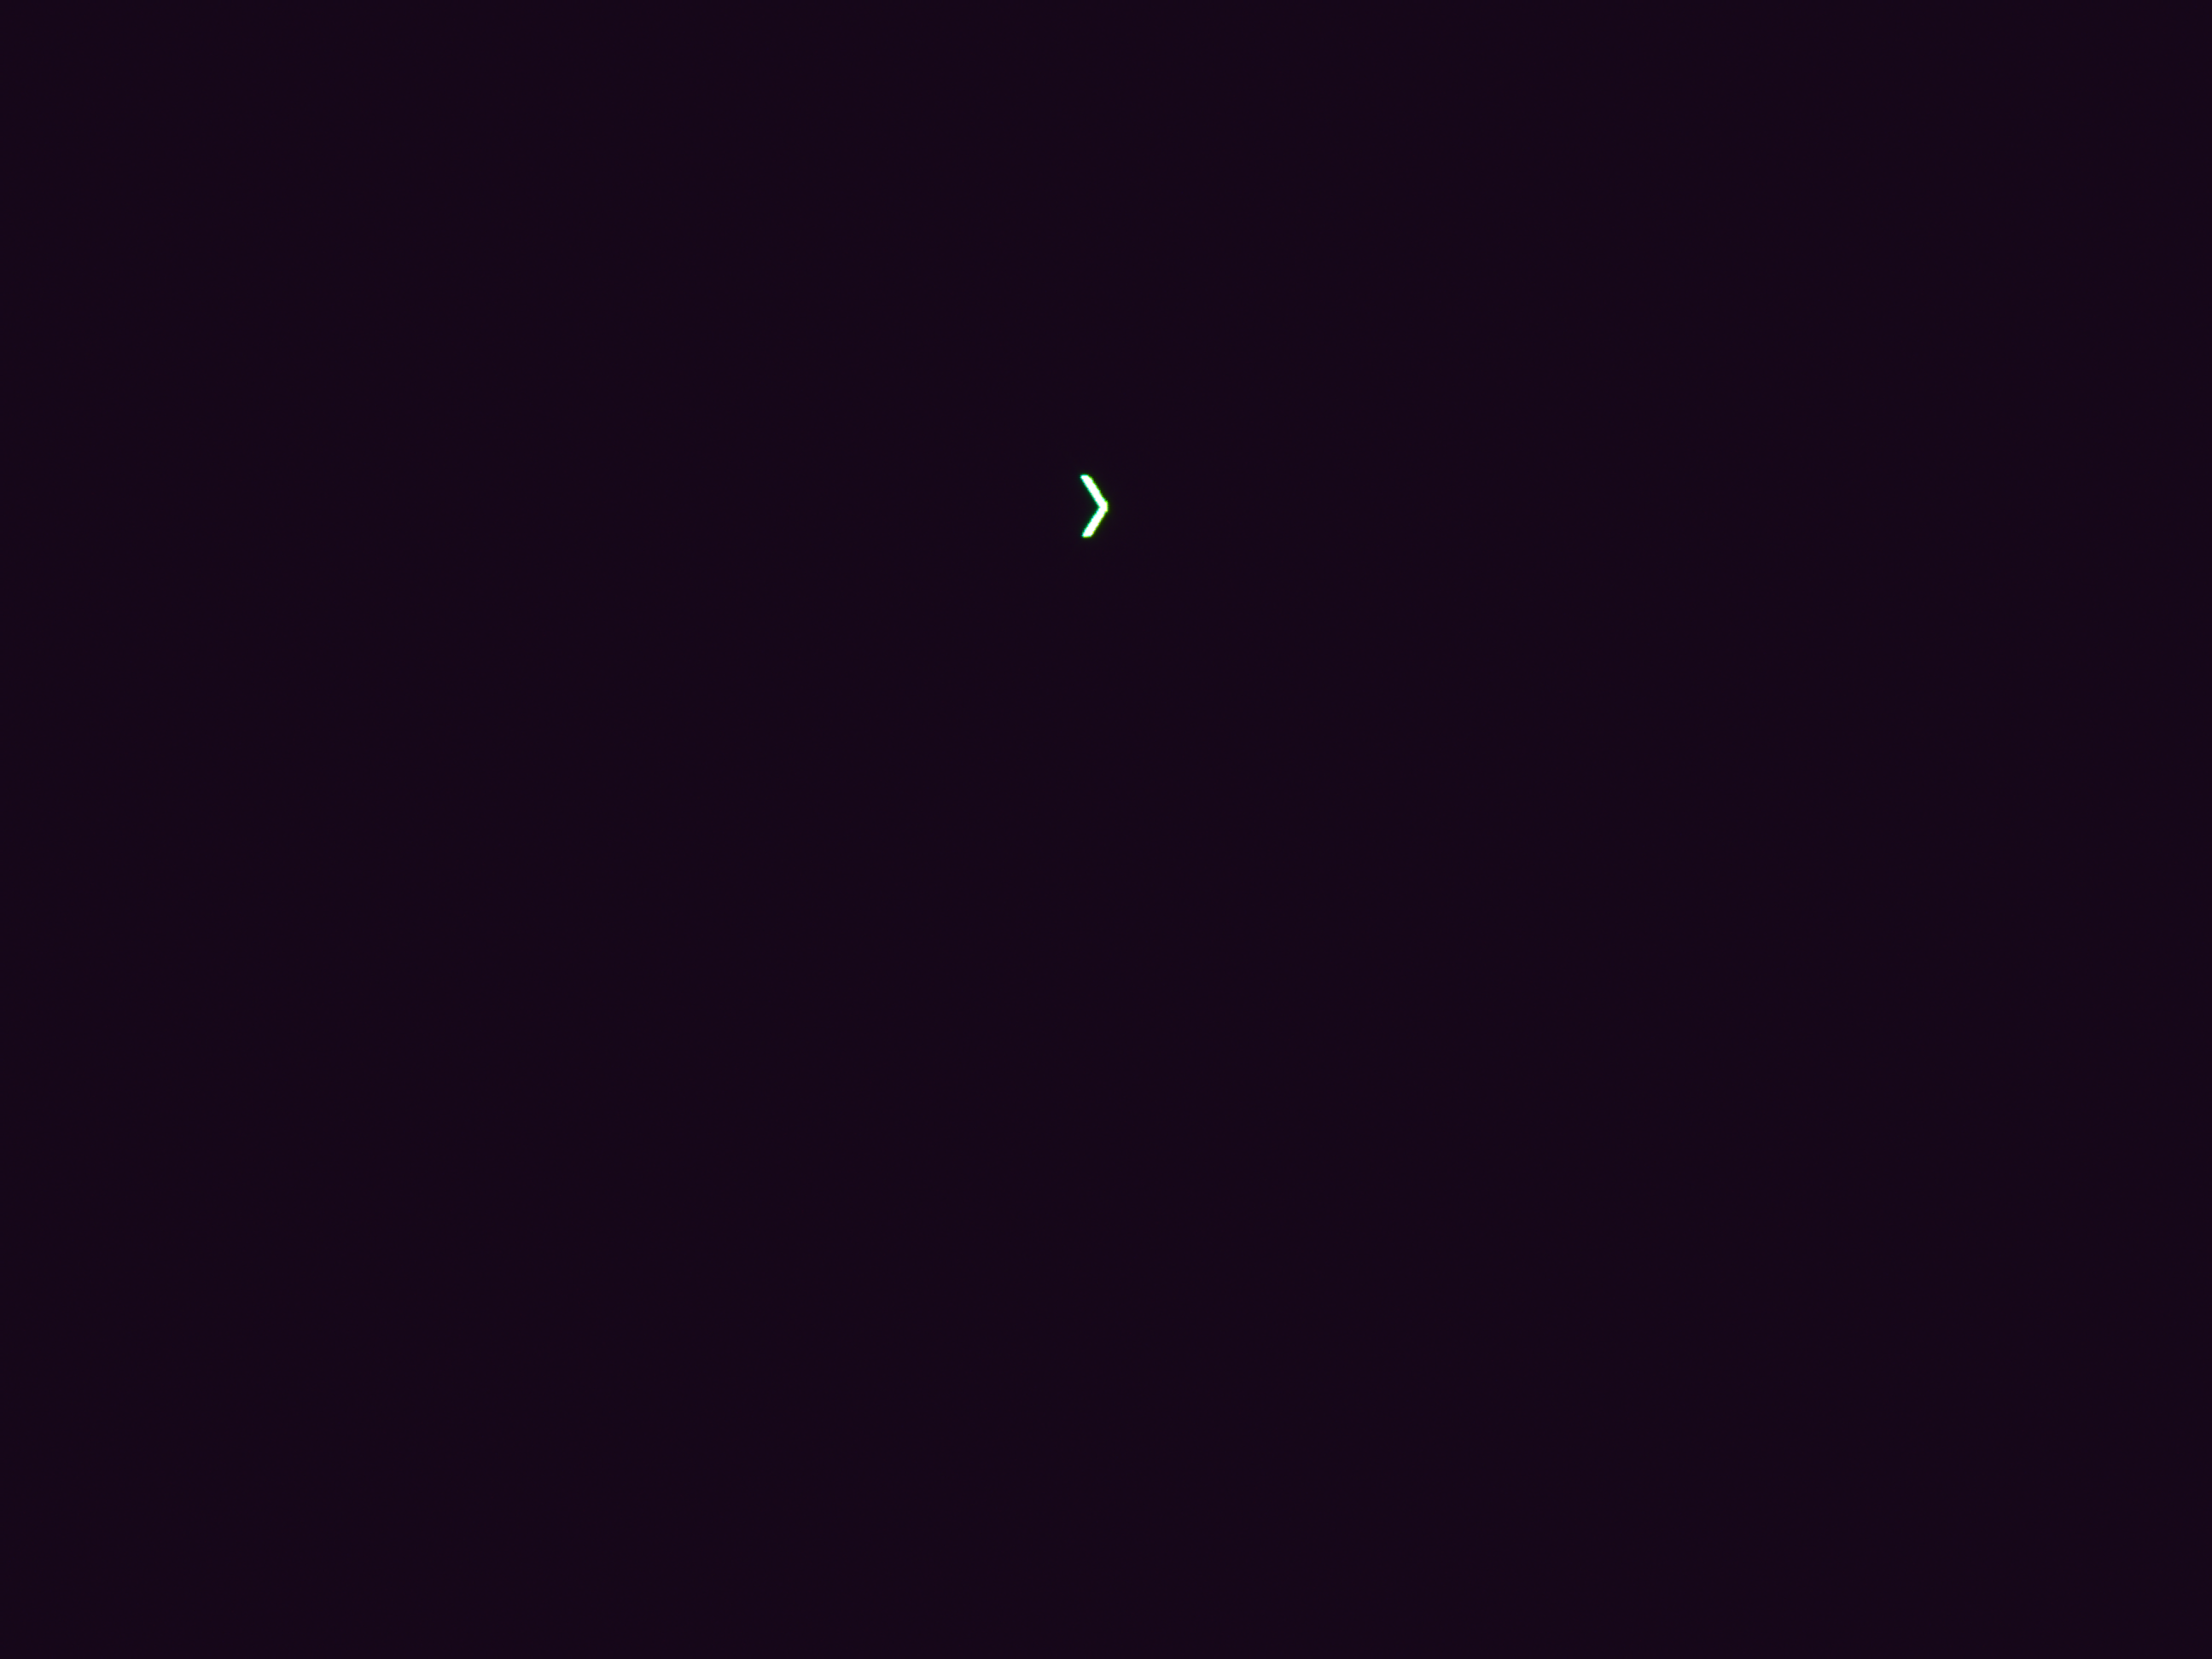
\includegraphics[width=\linewidth]{实验一/分析/参考物.png}
      \caption{参考物}
      \label{fig:点扩散函数参考物}
    \end{minipage}
    \hfill
    \begin{minipage}[b]{0.48\linewidth}
      \centering
      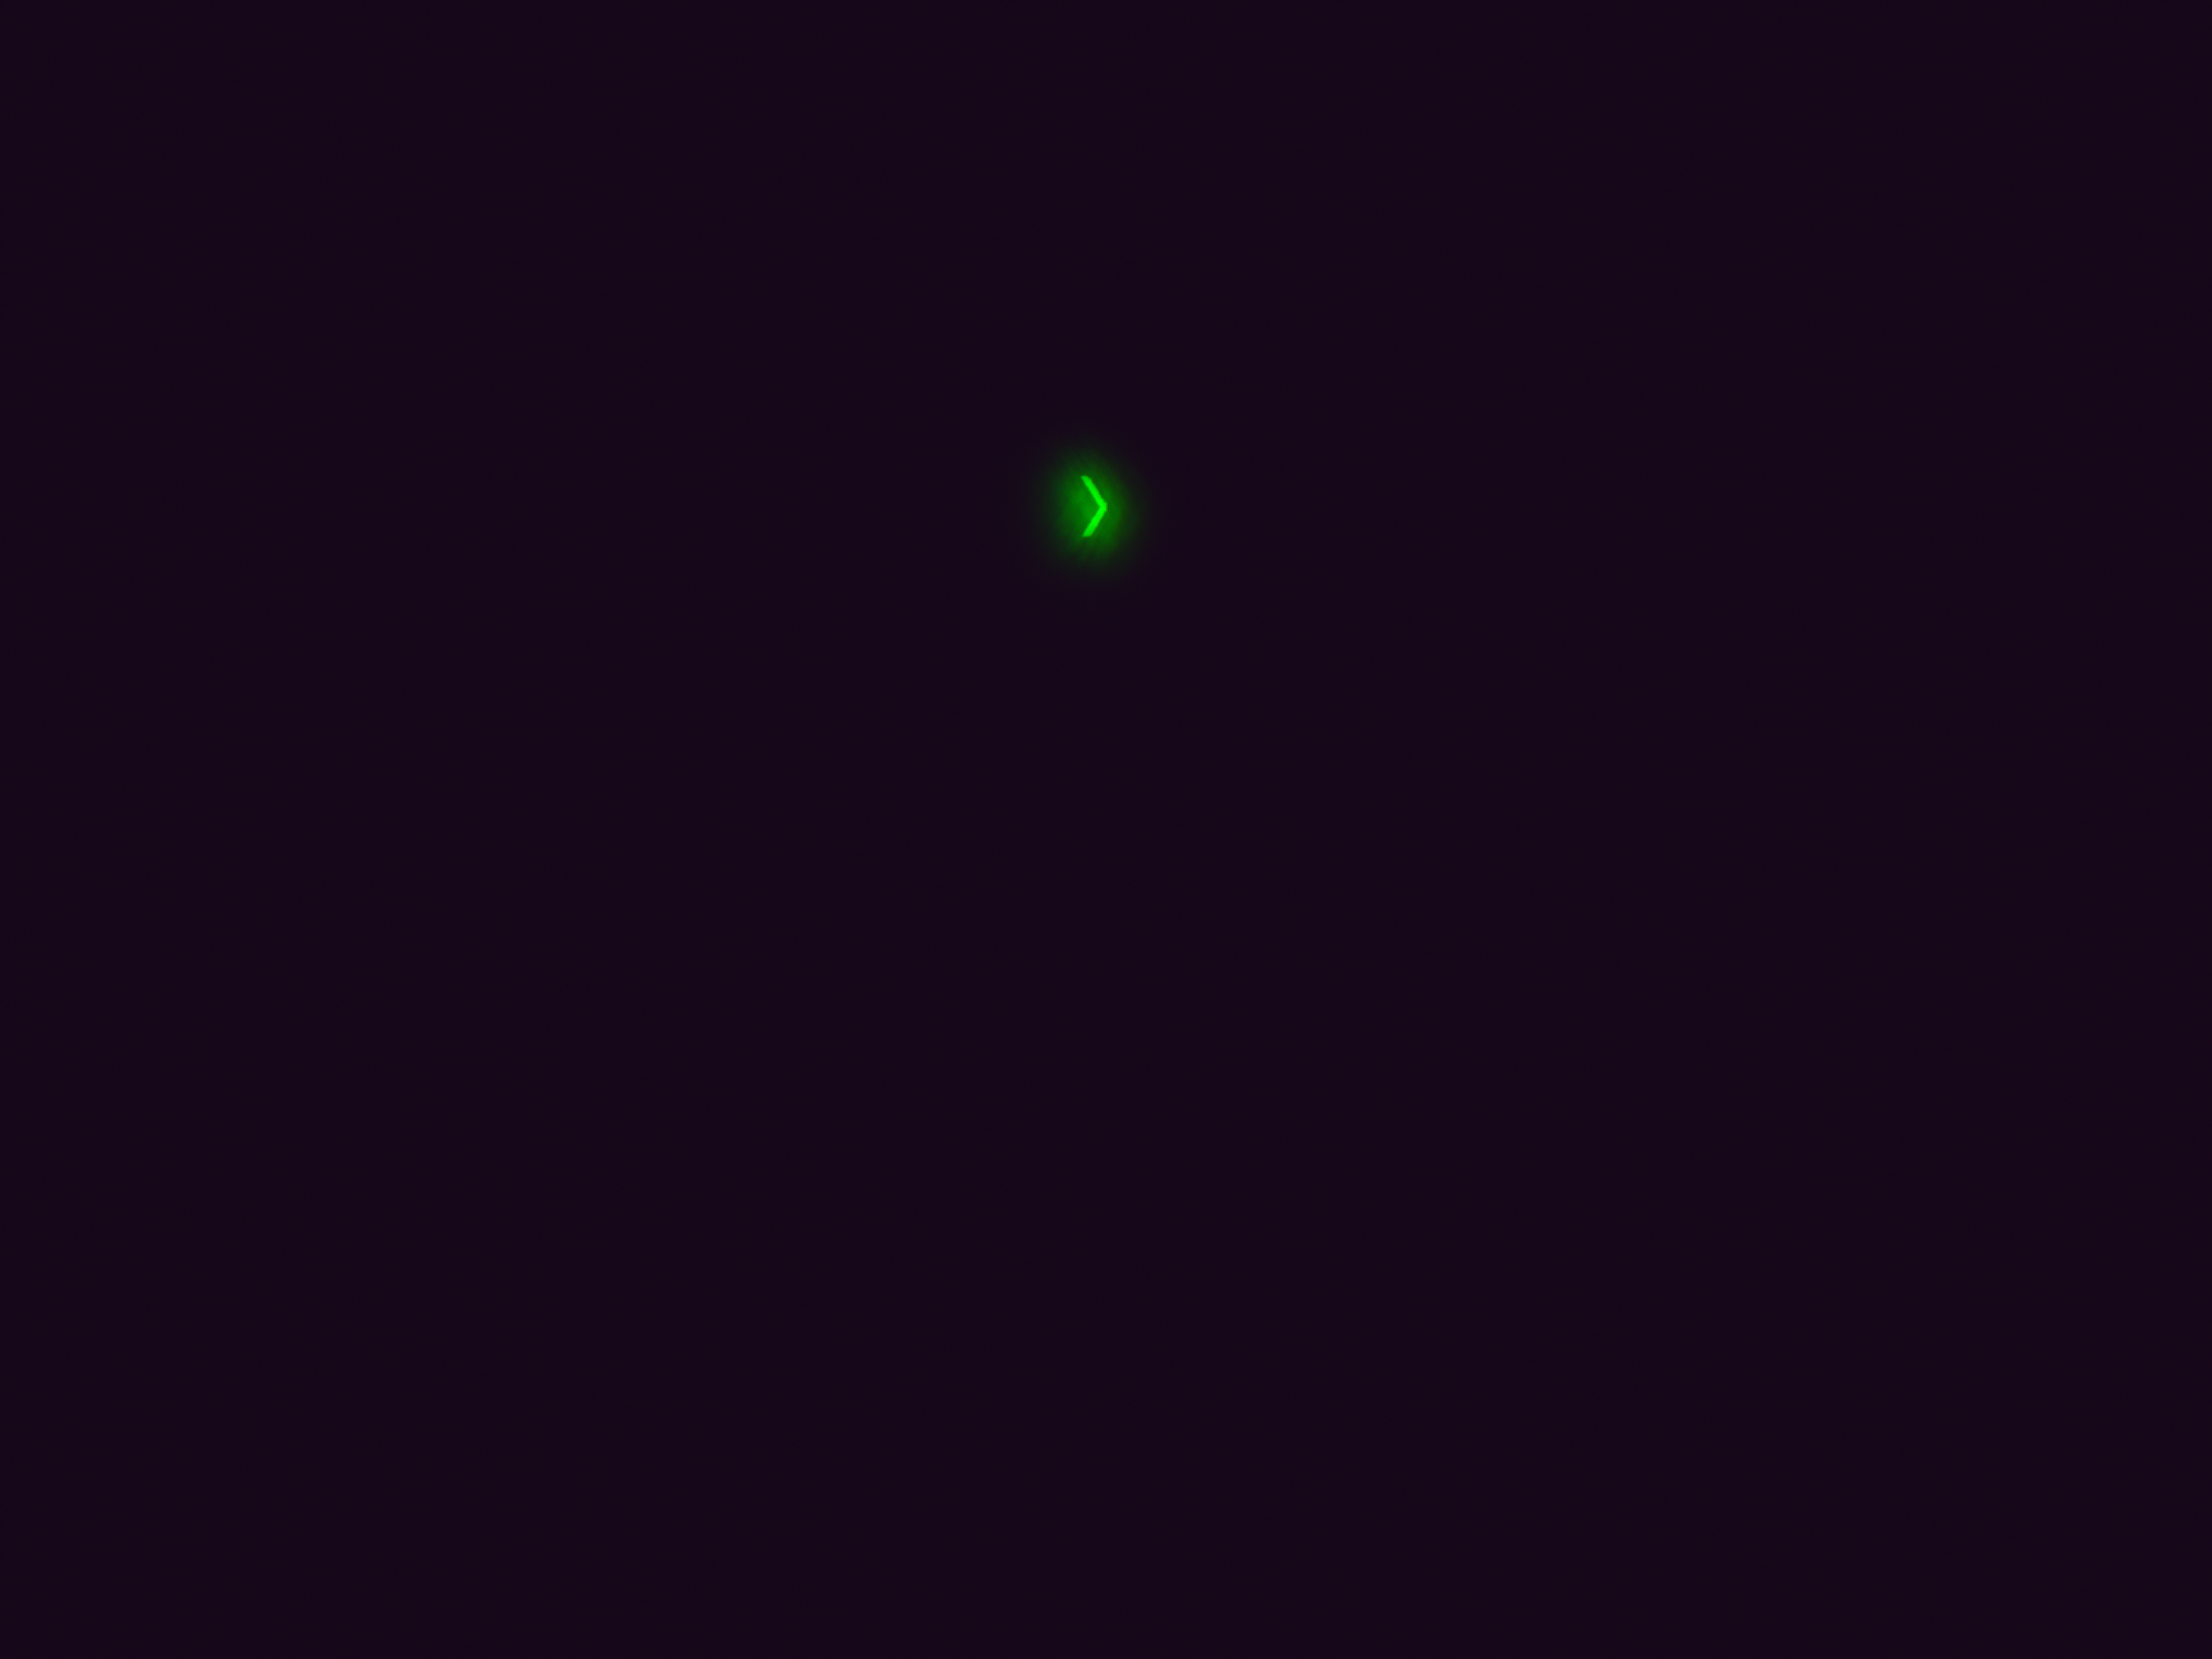
\includegraphics[width=\linewidth]{images/实验一/分析/参考散斑}
      \caption{参考散斑}
      \label{fig:点扩散函数参考散斑}
    \end{minipage}
  \end{figure}
  \begin{figure}[{H}]
    \centering
    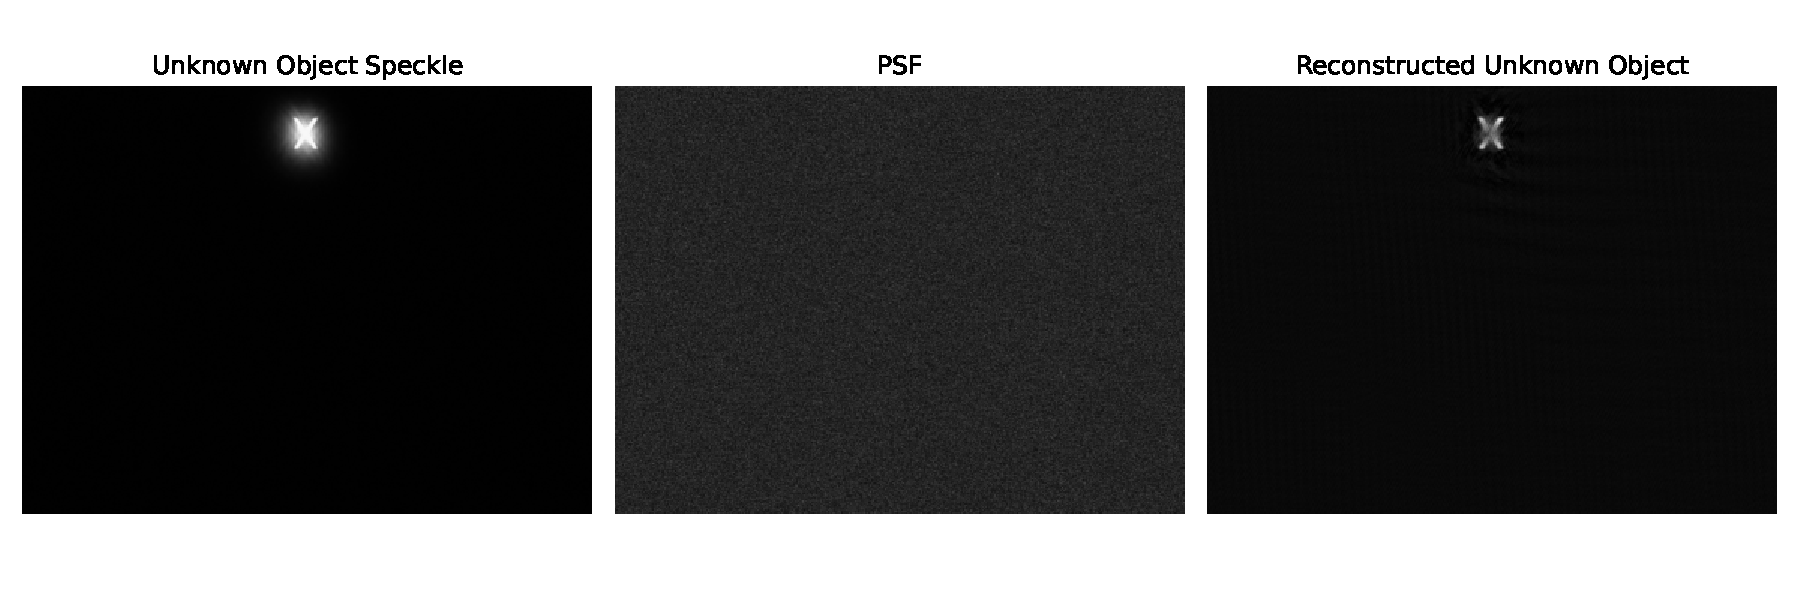
\includegraphics[width=0.8\linewidth]{images/实验一/分析/图像对比图.pdf}
    \caption{图像对比图}
    \label{fig:点扩散函数图像重建}
  \end{figure}




  我们首先将字母遮挡一半,作为参考物(\cref{fig:点扩散函数参考物})和参考散斑(\cref{fig:点扩散函数参考散斑}),用于求解点扩散函数;随后去掉遮挡,作为我们的未知物散斑,并使用刚刚求解的点扩散函数进行图像重建(\cref{fig:点扩散函数图像重建})。

  



\subsection{记忆效应范围测量}

  


  \begin{figure}[H]
      \centering
      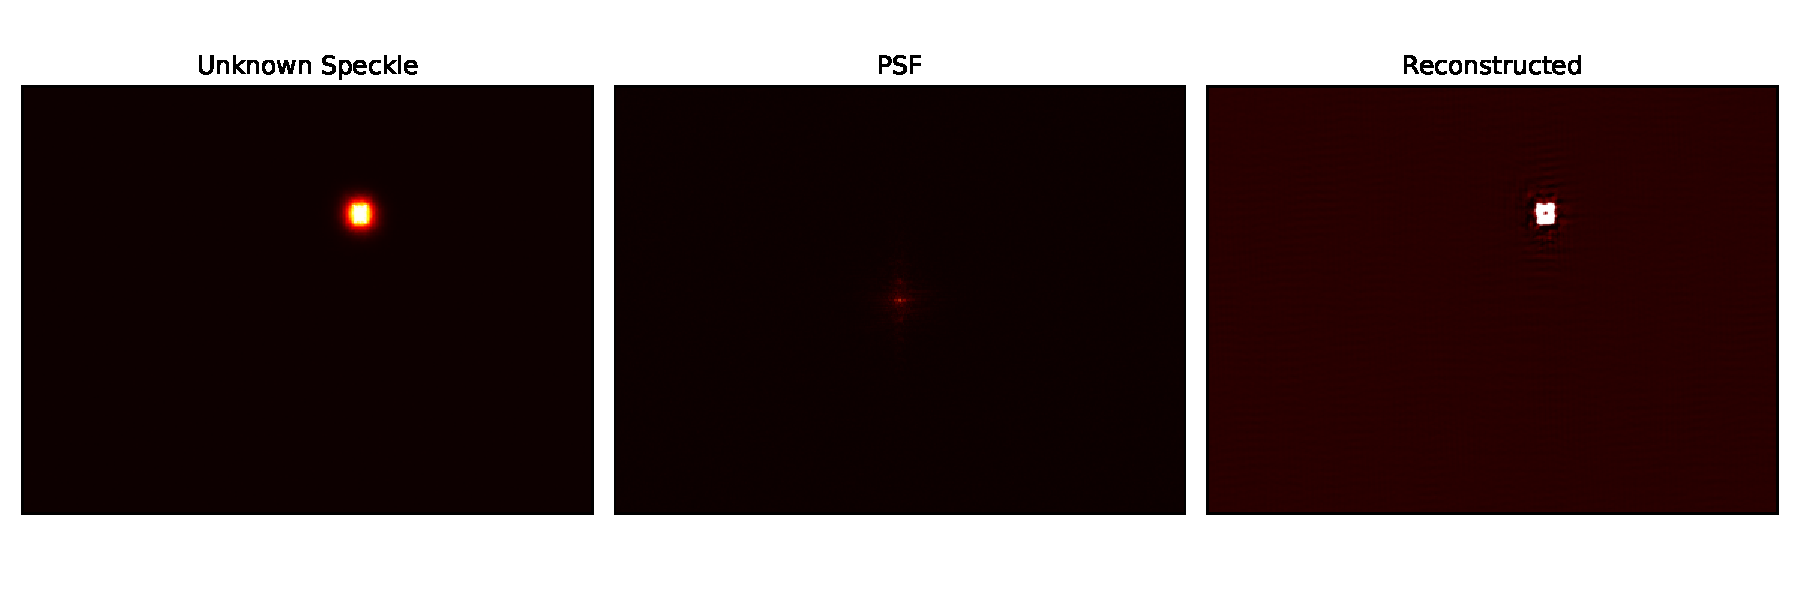
\includegraphics[width=0.8\linewidth]{实验一/-4mm/image_comparison.pdf}
      \caption{-4mm图像对比图}
      \label{fig:-4mm图像对比图}
  \end{figure}


  \begin{figure}[H]
      \centering
      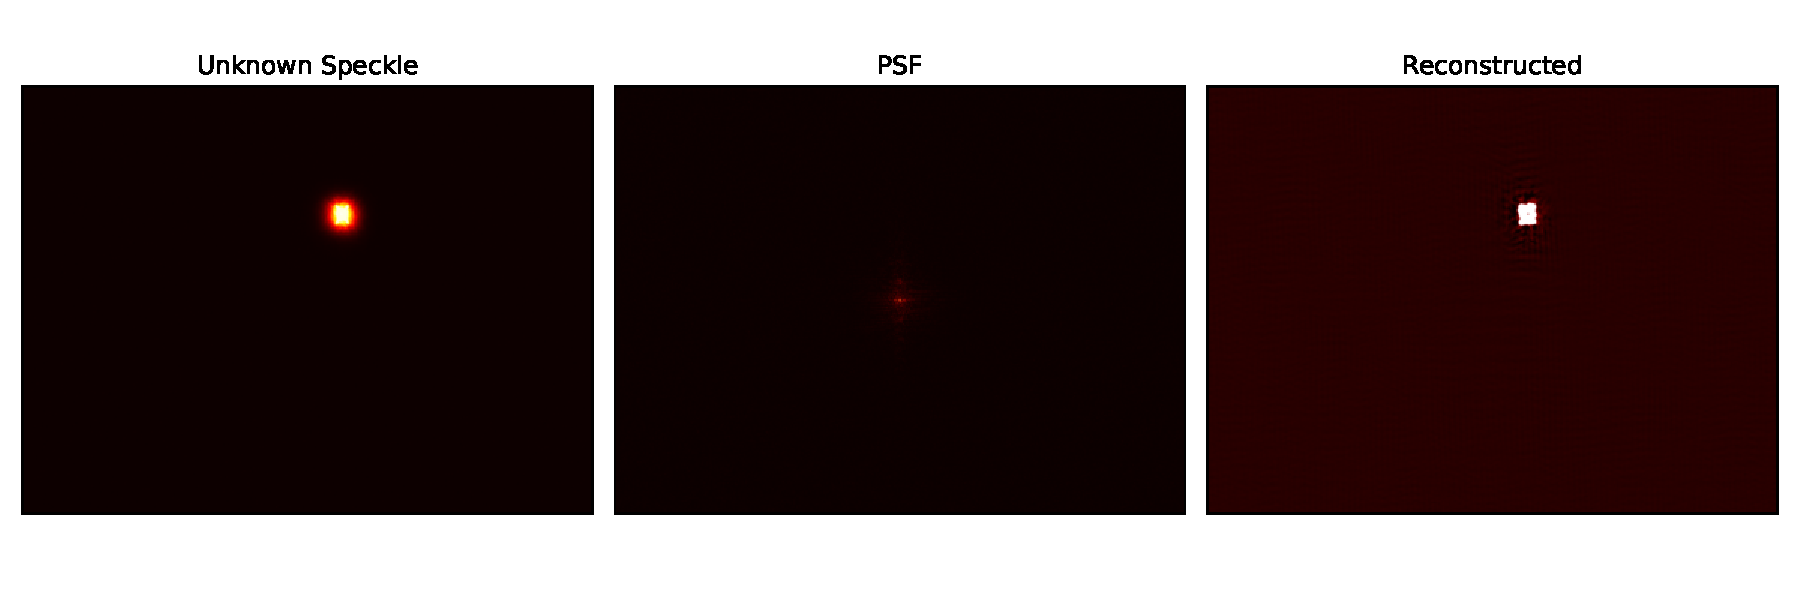
\includegraphics[width=0.8\linewidth]{实验一/-3mm/image_comparison.pdf}
      \caption{-3mm图像对比图}
      \label{fig:-3mm图像对比图}
  \end{figure}


  \begin{figure}[H]
      \centering
      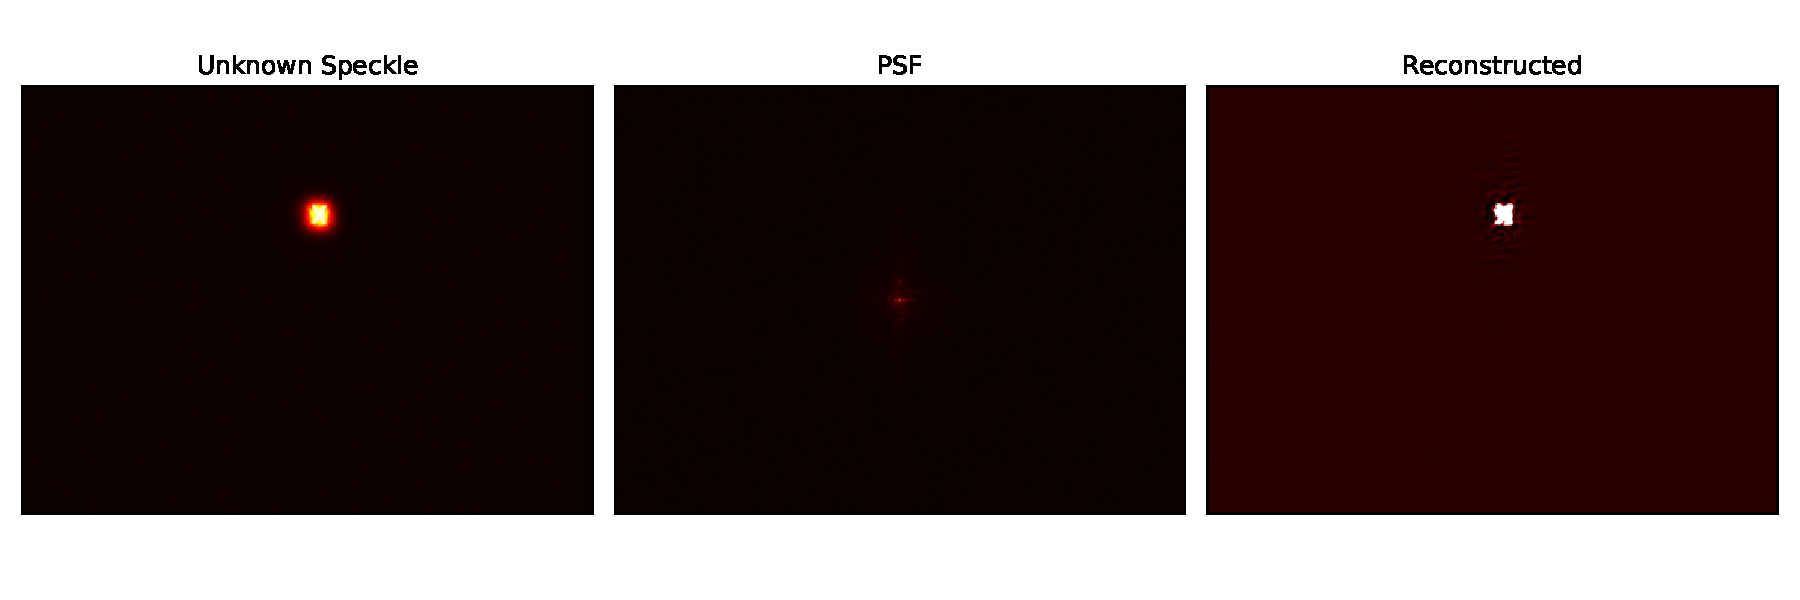
\includegraphics[width=0.8\linewidth]{实验一/-2mm/image_comparison.pdf}
      \caption{-2mm图像对比图}
      \label{fig:-2mm图像对比图}
  \end{figure}


  \begin{figure}[H]
      \centering
      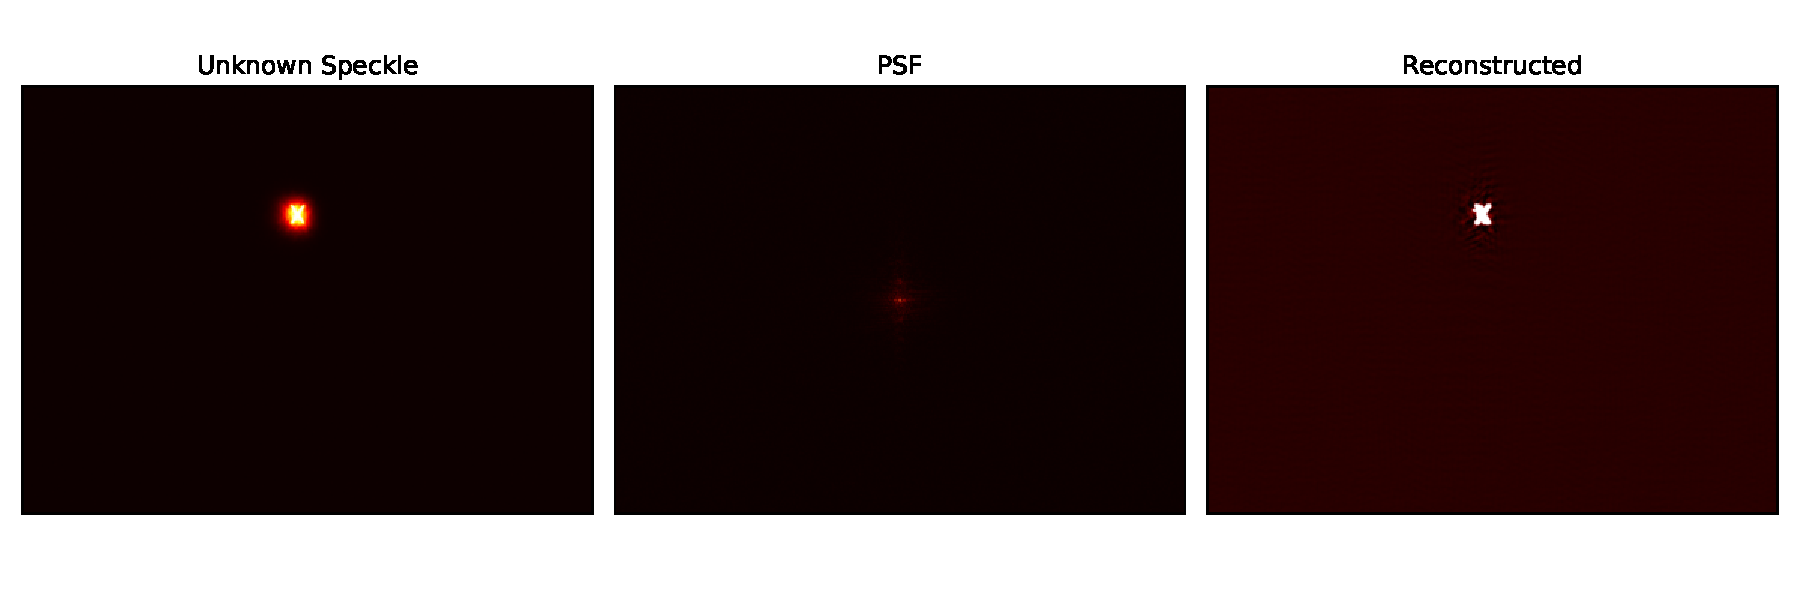
\includegraphics[width=0.8\linewidth]{实验一/-1mm/image_comparison.pdf}
      \caption{-1mm图像对比图}
      \label{fig:-1mm图像对比图}
  \end{figure}


  \begin{figure}[H]
      \centering
      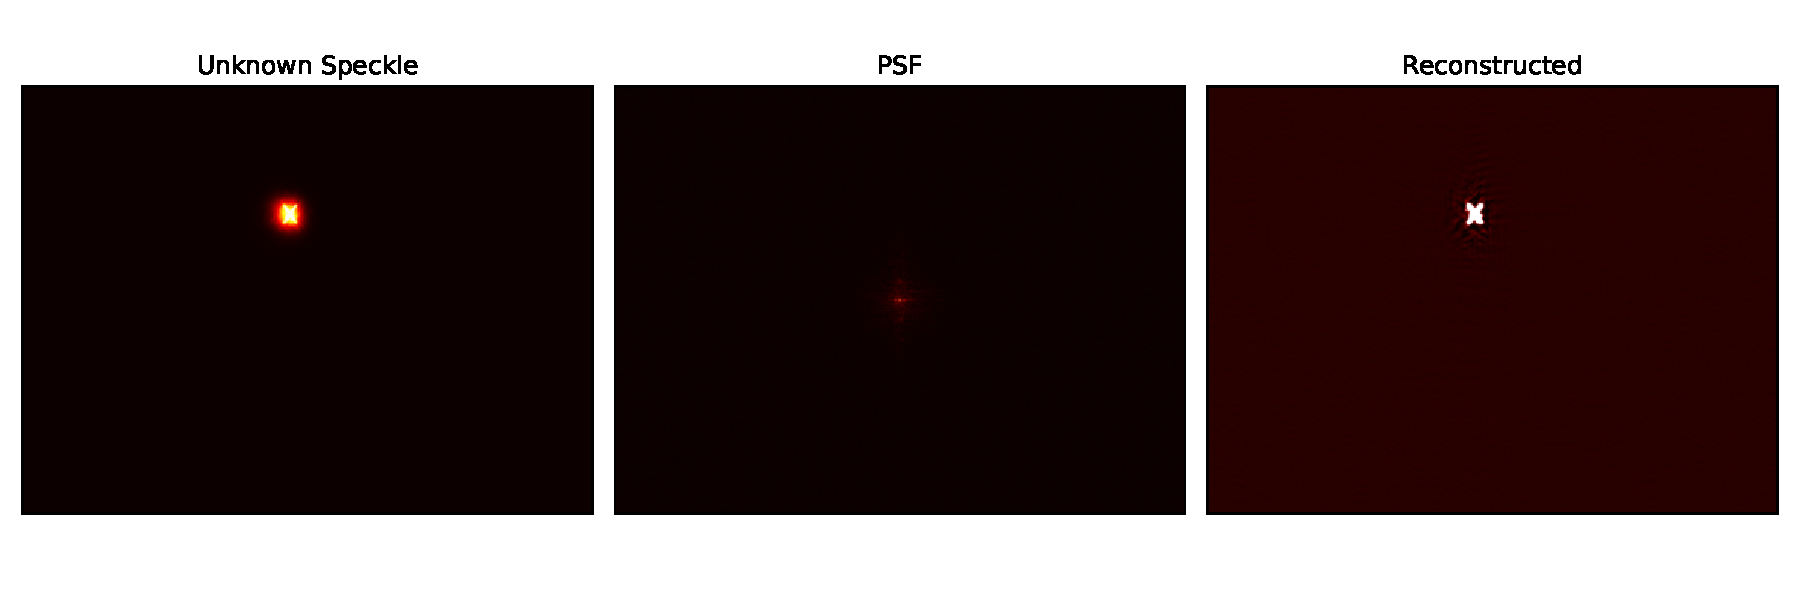
\includegraphics[width=0.8\linewidth]{实验一/0mm/image_comparison.pdf}
      \caption{0mm图像对比图}
      \label{fig:0mm图像对比图}
  \end{figure}


  \begin{figure}[H]
      \centering
      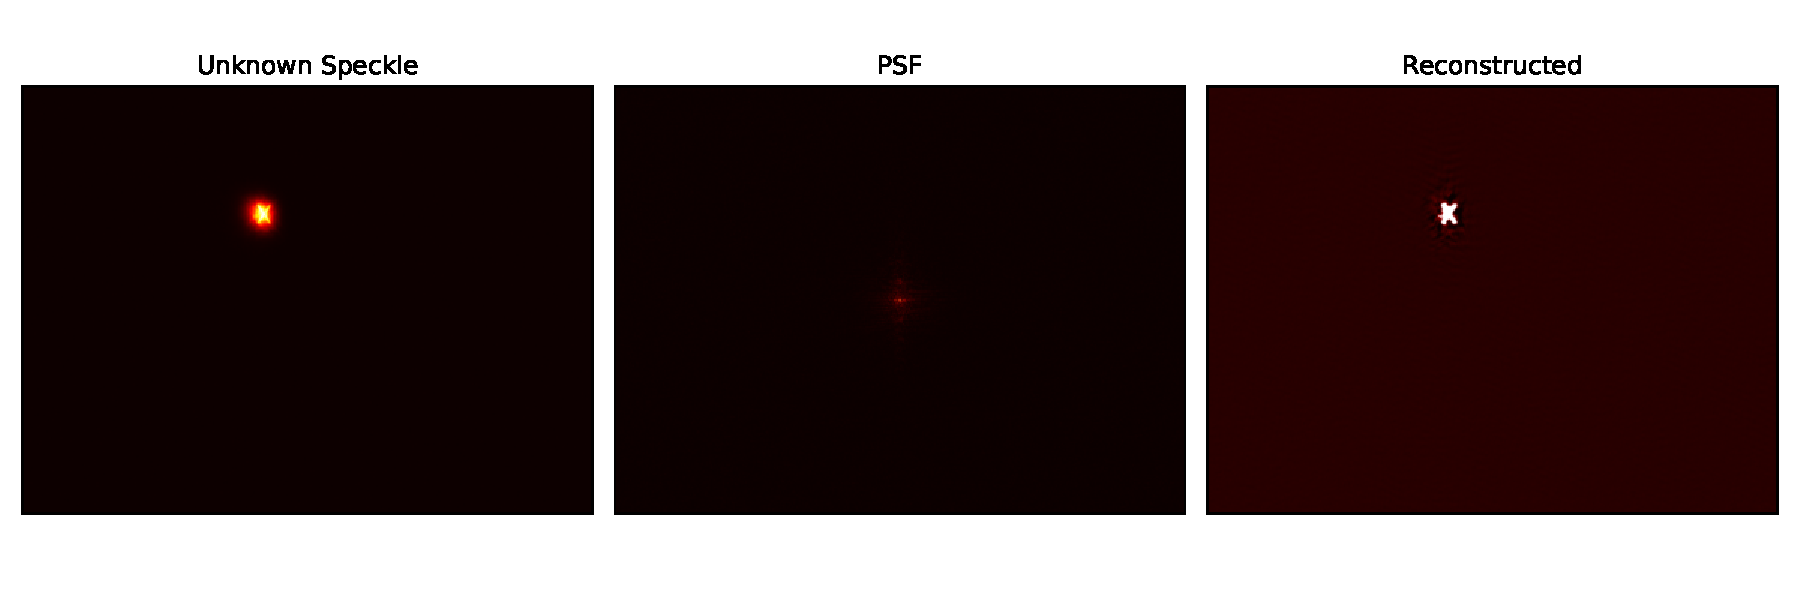
\includegraphics[width=0.8\linewidth]{实验一/+1mm/image_comparison.pdf}
      \caption{+1mm图像对比图}
      \label{fig:+1mm图像对比图}
  \end{figure}


  \begin{figure}[H]
      \centering
      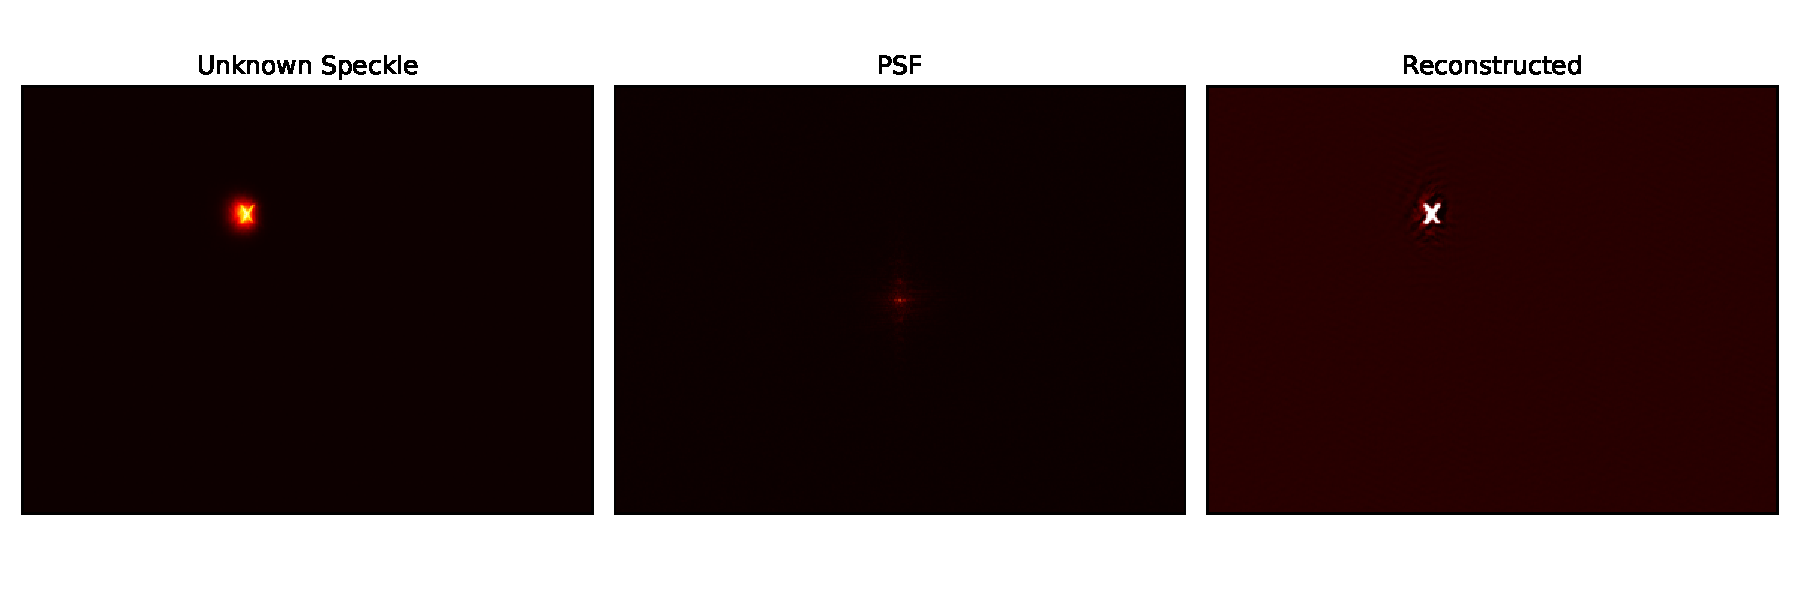
\includegraphics[width=0.8\linewidth]{实验一/+2mm/image_comparison.pdf}
      \caption{+2mm图像对比图}
      \label{fig:+2mm图像对比图}
  \end{figure}


  \begin{figure}[H]
      \centering
      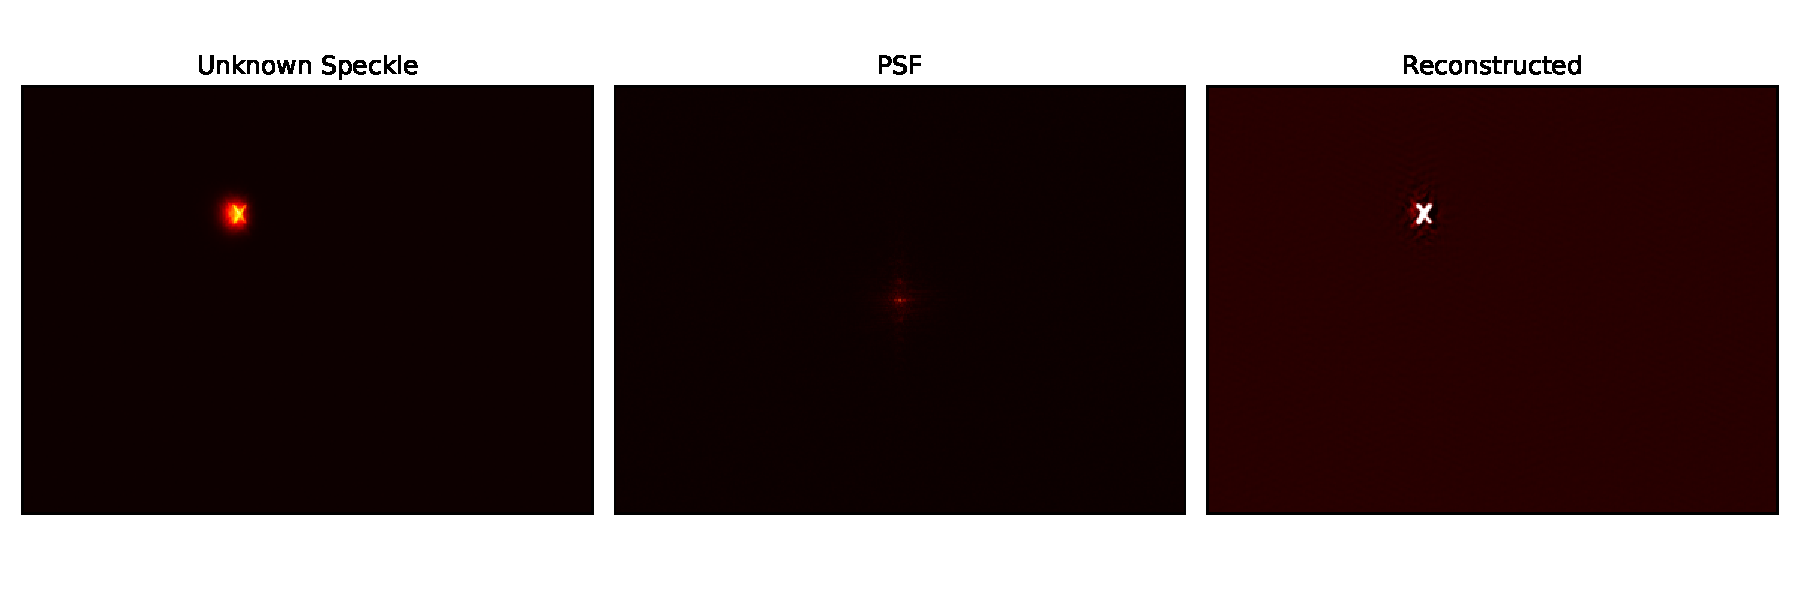
\includegraphics[width=0.8\linewidth]{实验一/+3mm/image_comparison.pdf}
      \caption{+3mm图像对比图}
      \label{fig:+3mm图像对比图}
  \end{figure}

  \begin{figure}[H]
      \centering
      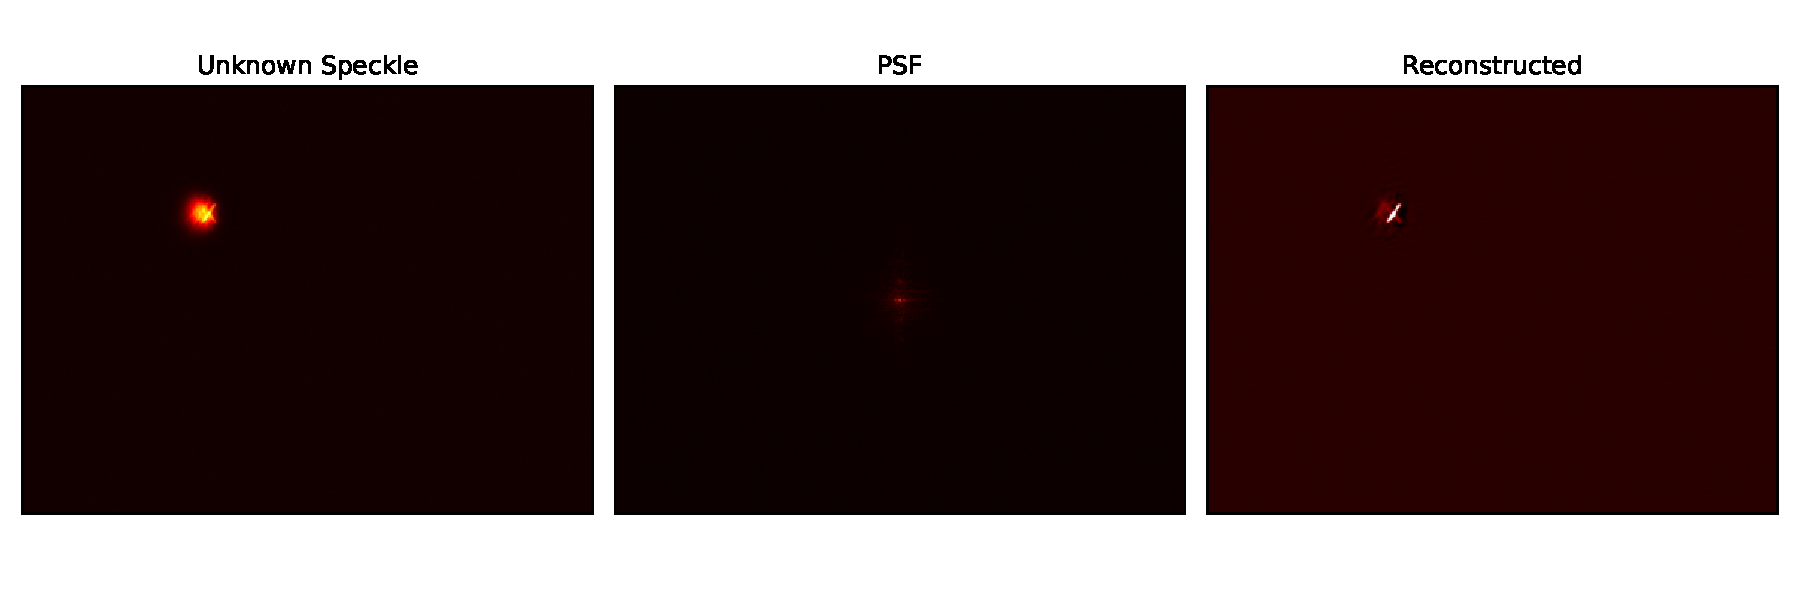
\includegraphics[width=0.8\linewidth]{实验一/+4mm/image_comparison.pdf}
      \caption{+4mm图像对比图}
      \label{fig:+4mm图像对比图}
  \end{figure}


  在记忆效应范围测量实验中,我们将字母板左右平移,分别测量不同位置的散斑,并使用\textbf{未平移}时所求解的点扩散函数进行图像重建,结果如(\cref{fig:-4mm图像对比图}--\cref{fig:+4mm图像对比图})所示。

  观察重建图像的效果可知,在平移范围在 ($\Delta x \in (-1, +3) $mm)内,图像重建效果均较好,说明该光学系统的记忆效应范围大约为($\pm 2$mm)。

  但是我们发现,该记忆效应范围区间没有关于 0 对称,这是因为我们的字母在 “0mm” 位置时并不在光轴上。

% 对于记忆效应的测量,观察图像可知,在1mm范围内,可以观察到恢复图像的效果较好,在1mm之外就会出现无法分辨出原始字母的情况,可以认定为:记忆效应的范围为1mm。




\subsection{实验二:散射光成像的影响条件}

\subsubsection{旋转记忆效应}
% ============ 旋转记忆效应 ============
  % 大角度旋转
  \begin{figure}[H]
      \centering
      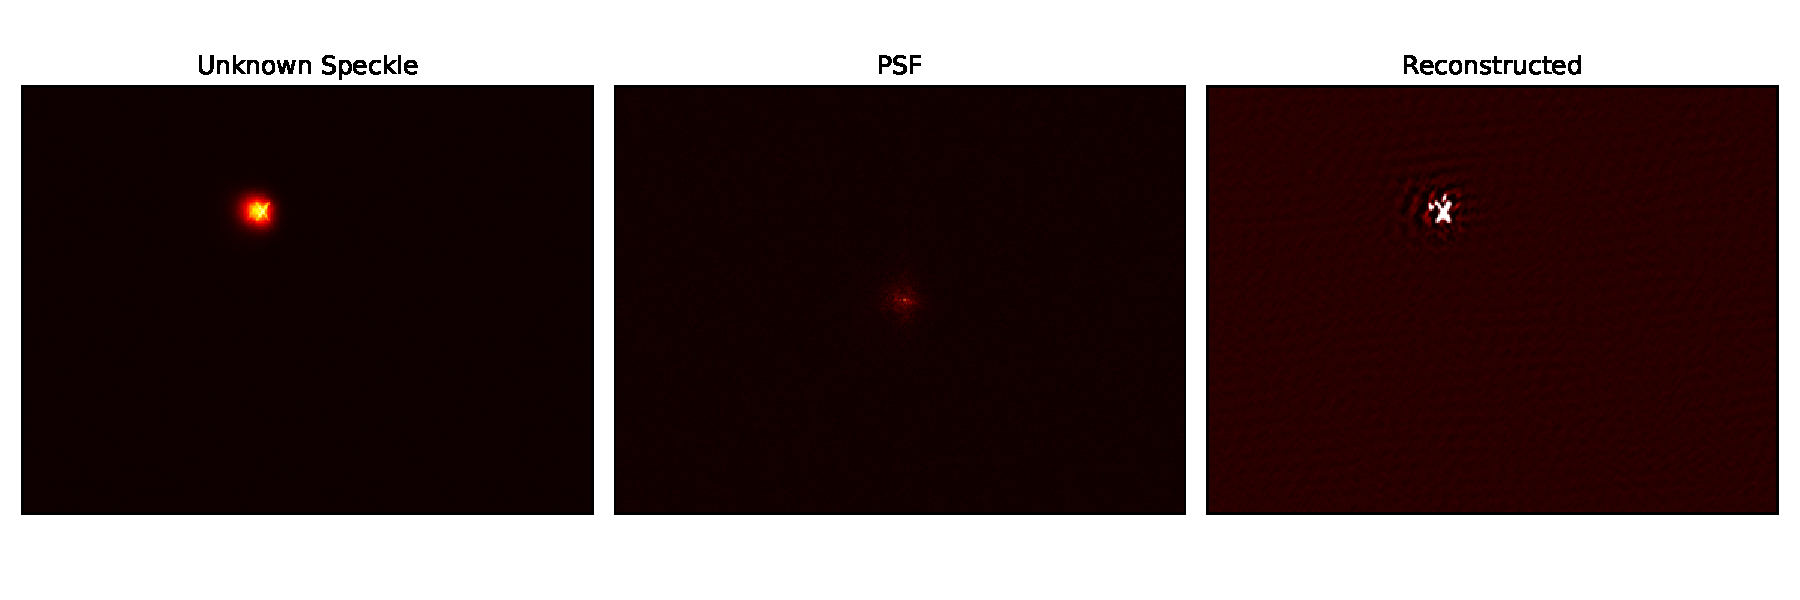
\includegraphics[width=0.8\linewidth]{实验二/旋转记忆效应/大角度旋转/图像对比图.pdf}
      \caption{大角度旋转图像对比图}
  \end{figure}

  % 小角度旋转
  \begin{figure}[H]
      \centering
      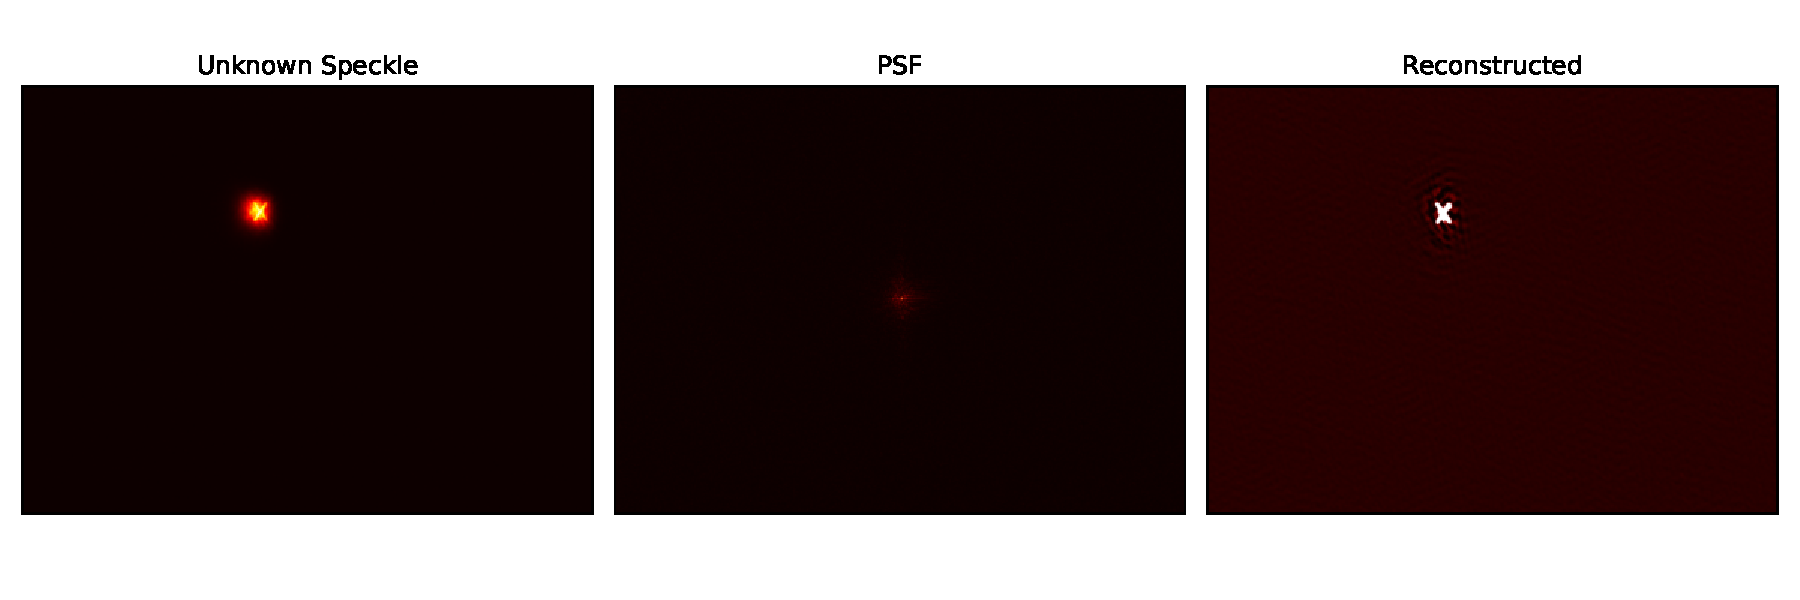
\includegraphics[width=0.8\linewidth]{实验二/旋转记忆效应/小角度旋转/图像对比图.pdf}
      \caption{小角度旋转图像对比图}
  \end{figure}

  旋转记忆效应是指当散射片绕垂直于光传播方向的轴发生微小旋转时,出射散斑图不会完全改变,而是整体发生旋转,保持一定的空间相关性。在实验中轻轻旋转散射片时图像仍能重建,说明系统处于旋转记忆效应有效范围内;但若旋转角度过大,相关性丧失,重建将失败。因此,适度旋转下的成像稳定性体现了散射系统的旋转记忆能力。

  根据实验结果来看,小角度和大角度均可以分辨出图像,但是从效果上来看,小角度的成像效果是优于大角度的。






\subsubsection{焦距的影响}
% ============ 焦距的影响 ============
  % 工作距离50 - 焦距18mm
  \begin{figure}[H]
      \centering
      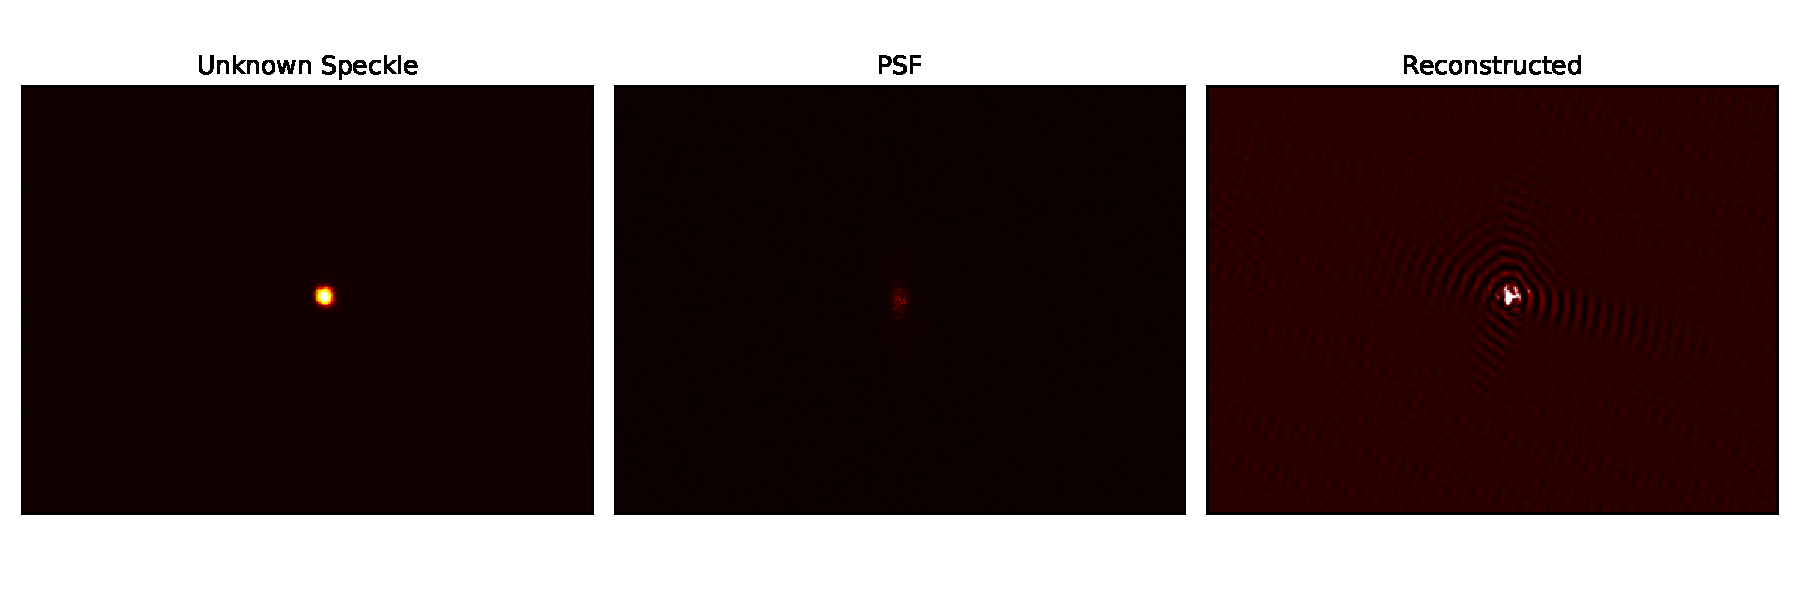
\includegraphics[width=0.8\linewidth]{实验二/焦距的影响/工作距离50/焦距18/图像对比图.pdf}
      \caption{工作距离50cm-焦距18mm图像对比图}
  \end{figure}

  % 工作距离50 - 焦距40mm
  \begin{figure}[H]
      \centering
      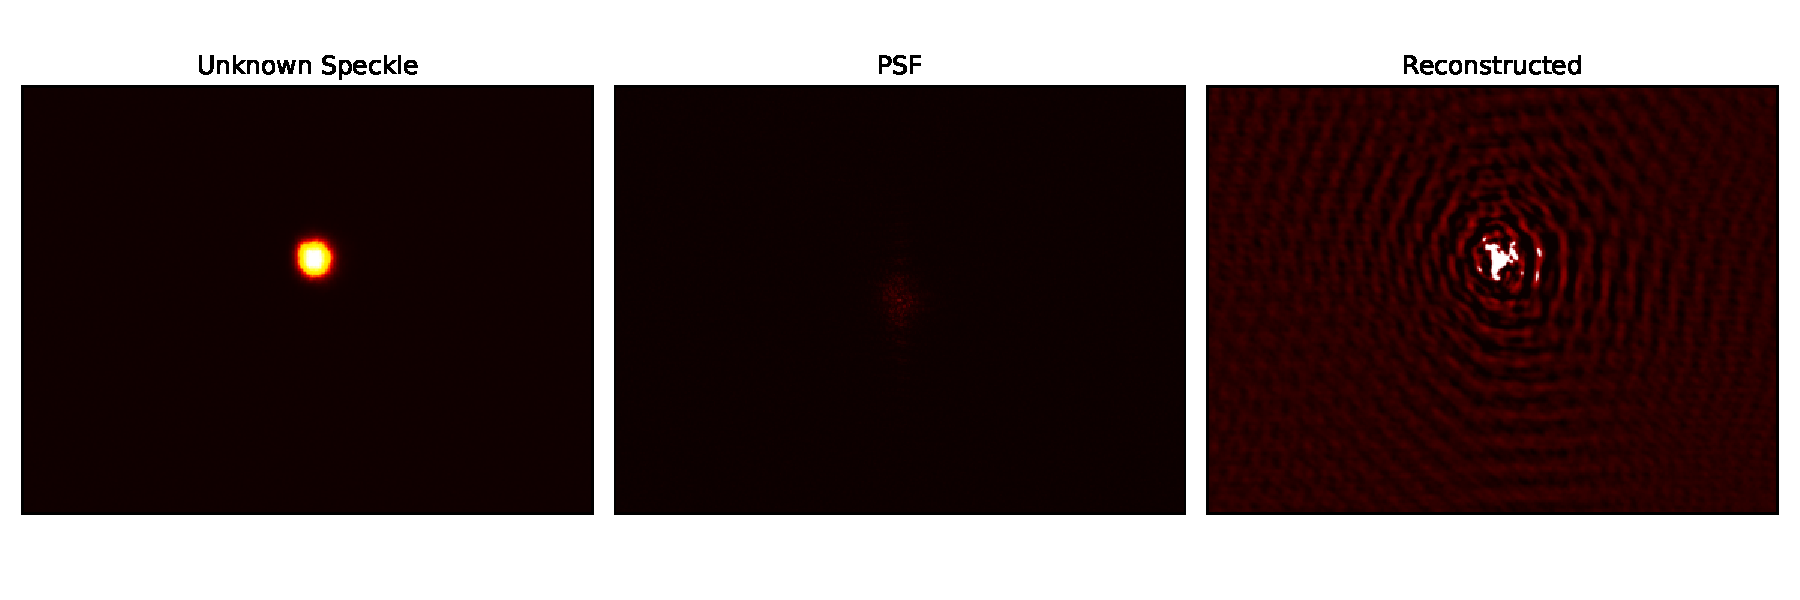
\includegraphics[width=0.8\linewidth]{实验二/焦距的影响/工作距离50/焦距40/图像对比图.pdf}
      \caption{工作距离50cm-焦距40mm图像对比图}
  \end{figure}

  % 工作距离50 - 焦距108mm
  \begin{figure}[H]
      \centering
      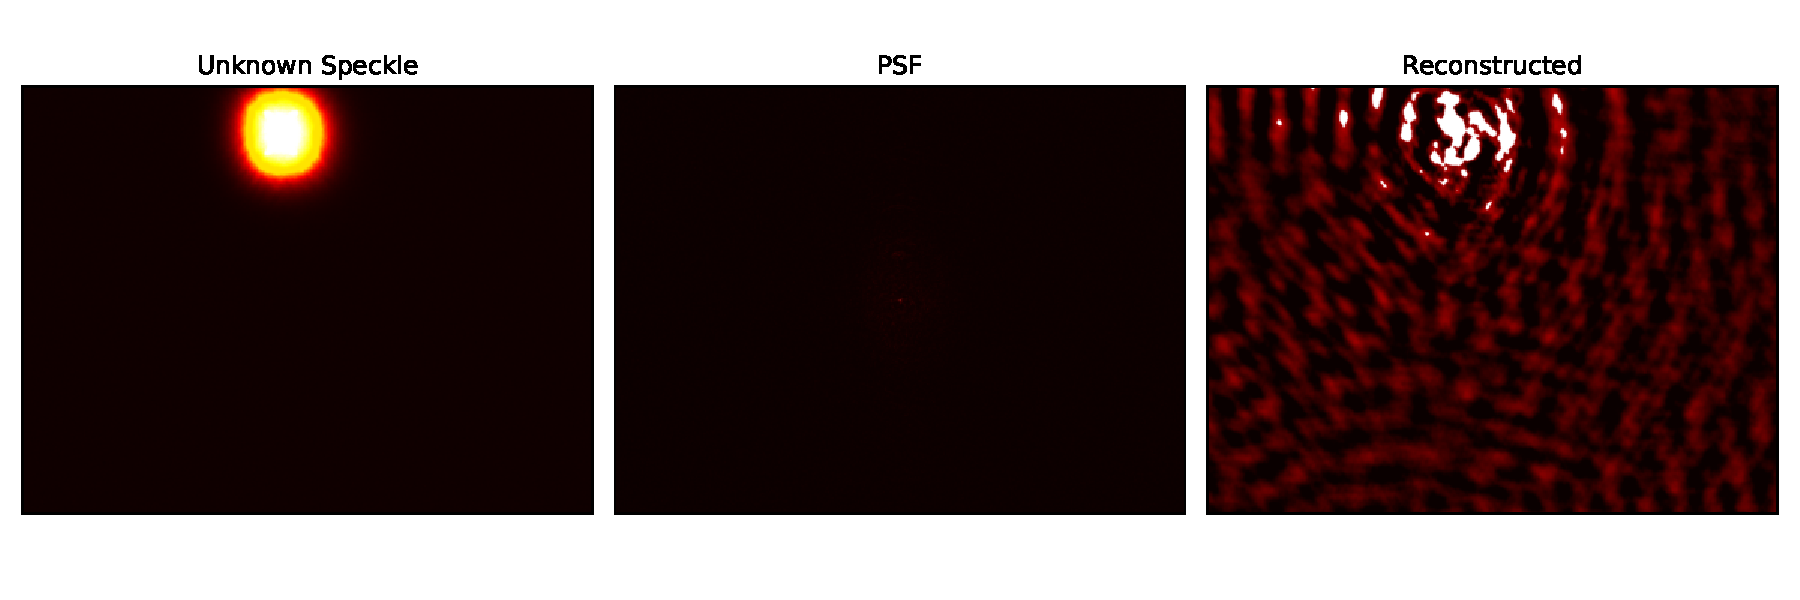
\includegraphics[width=0.8\linewidth]{实验二/焦距的影响/工作距离50/焦距108/图像对比图.pdf}
      \caption{工作距离50cm-焦距108mm图像对比图}
  \end{figure}

  % 工作距离68cm - 焦距18mm
  \begin{figure}[H]
      \centering
      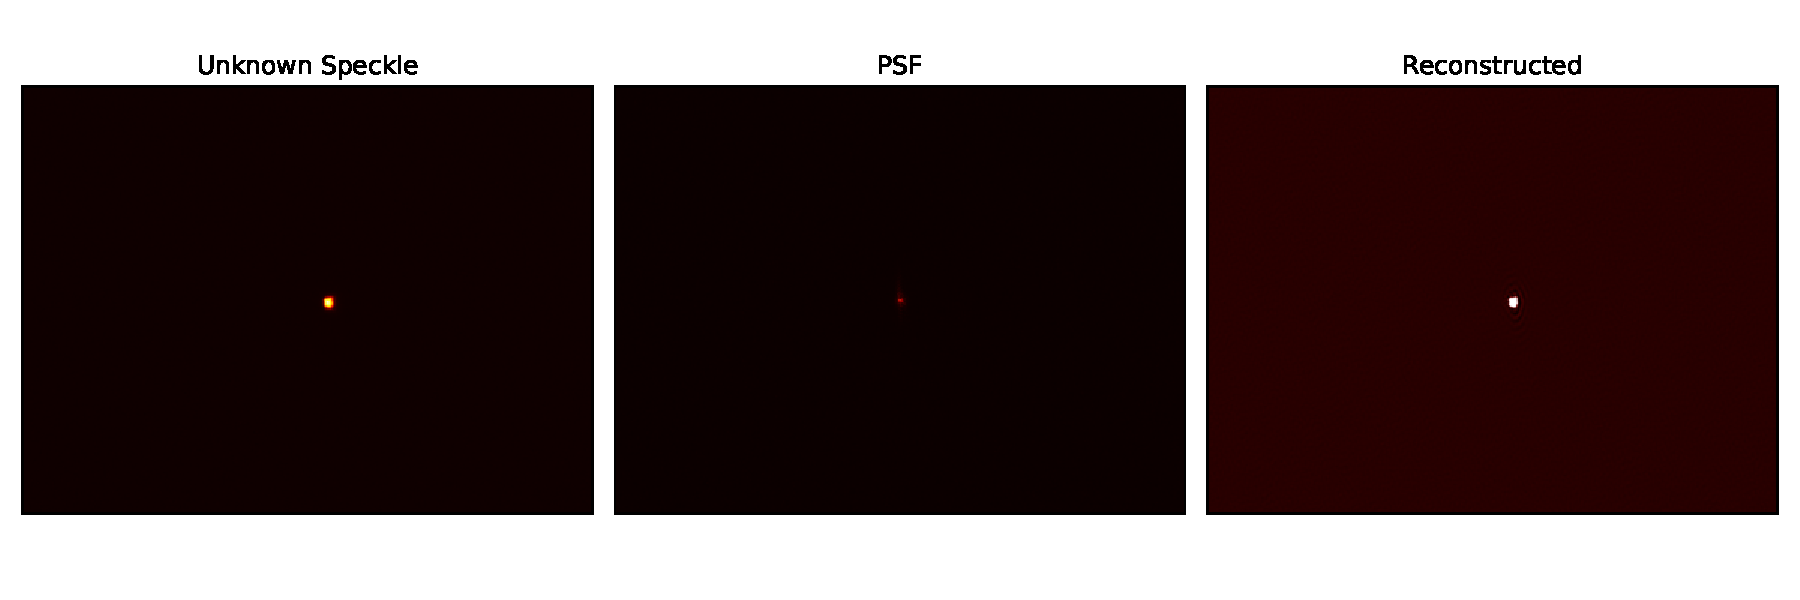
\includegraphics[width=0.8\linewidth]{实验二/焦距的影响/工作距离68/焦距18/图像对比图.pdf}
      \caption{工作距离68cm-焦距18mm图像对比图}
  \end{figure}

  % 工作距离68cm - 焦距40mm
  \begin{figure}[H]
      \centering
      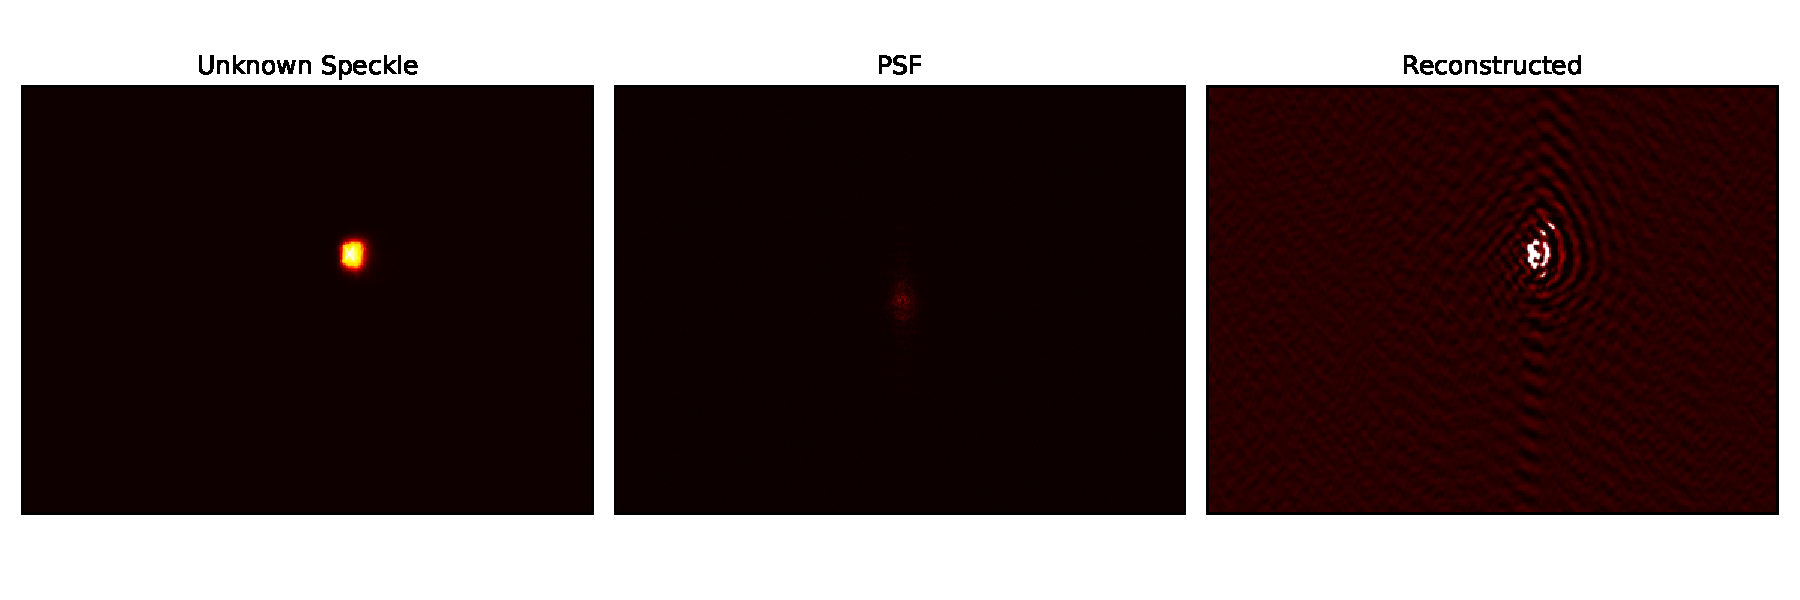
\includegraphics[width=0.8\linewidth]{实验二/焦距的影响/工作距离68/焦距40/图像对比图.pdf}
      \caption{工作距离68cm-焦距40mm图像对比图}
  \end{figure}

  % 工作距离68cm - 焦距108mm
  \begin{figure}[H]
      \centering
      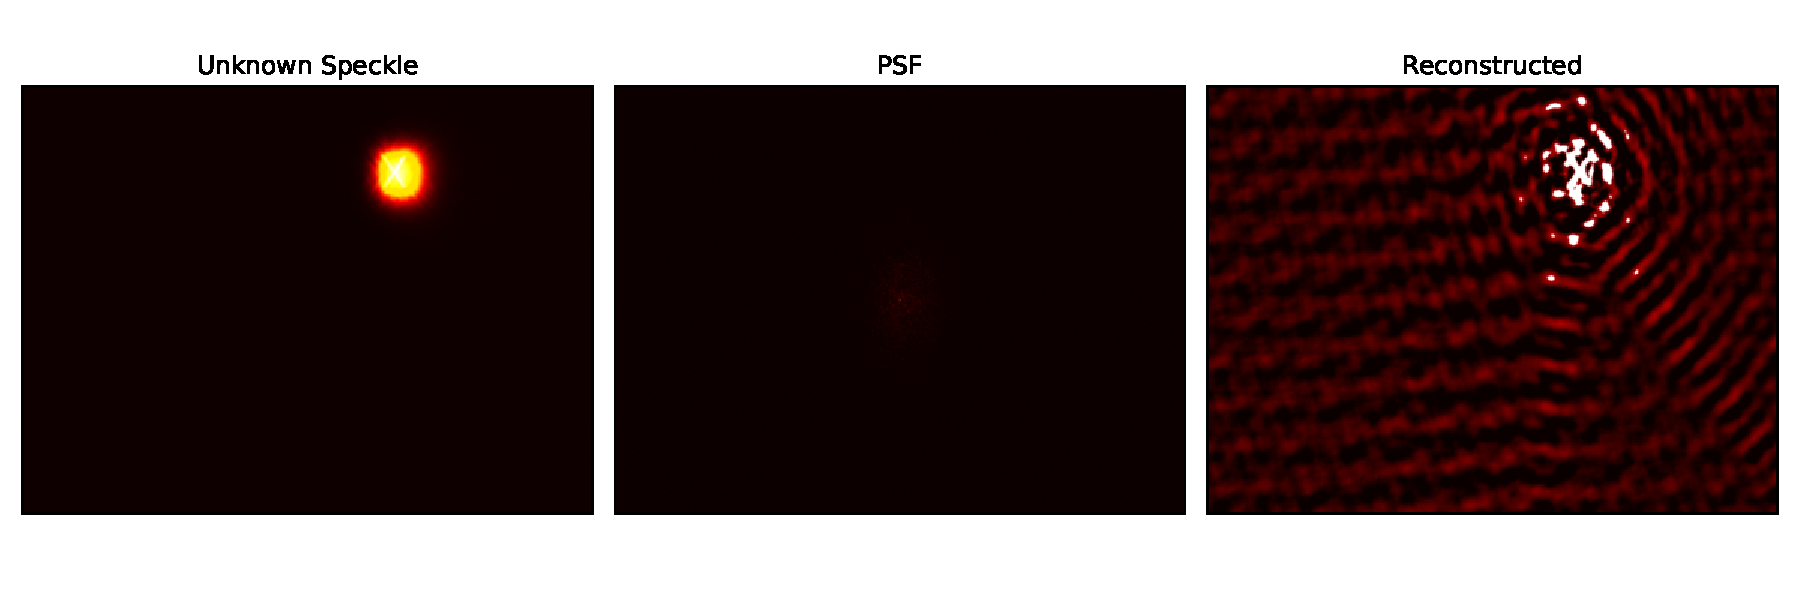
\includegraphics[width=0.8\linewidth]{实验二/焦距的影响/工作距离68/焦距108/图像对比图.pdf}
      \caption{工作距离68cm-焦距108mm图像对比图}
  \end{figure}


  镜头焦距决定了成像系统的放大倍率和视场大小,从而影响对散斑图的采集能力。在散射光成像中,较短焦距提供较大的视场和更高的光通量,有助于获取完整的散斑图结构,但角度分辨率较低,不利于微小扰动下的成像重建;而较长焦距则提高了角度分辨率和对细节的敏感性,使记忆效应下散斑图的微小位移更加明显,有利于图像恢复,但光强降低、视场变小,对系统稳定性要求更高。因此,焦距的选择需在视场范围、分辨能力与信噪比之间权衡,以获得最佳重建效果。

  观察我们的数据可知,我们选择不同的焦距均没有成功重建图像,主要是因为在改变不同实验条件时,没有调整为共轴。







  
\subsubsection{工作距离}
% ============ 工作距离的影响 ============

  \begin{itemize}
    \item 第一次实验

      % 工作距离50cm
      \begin{figure}[H]
          \centering
          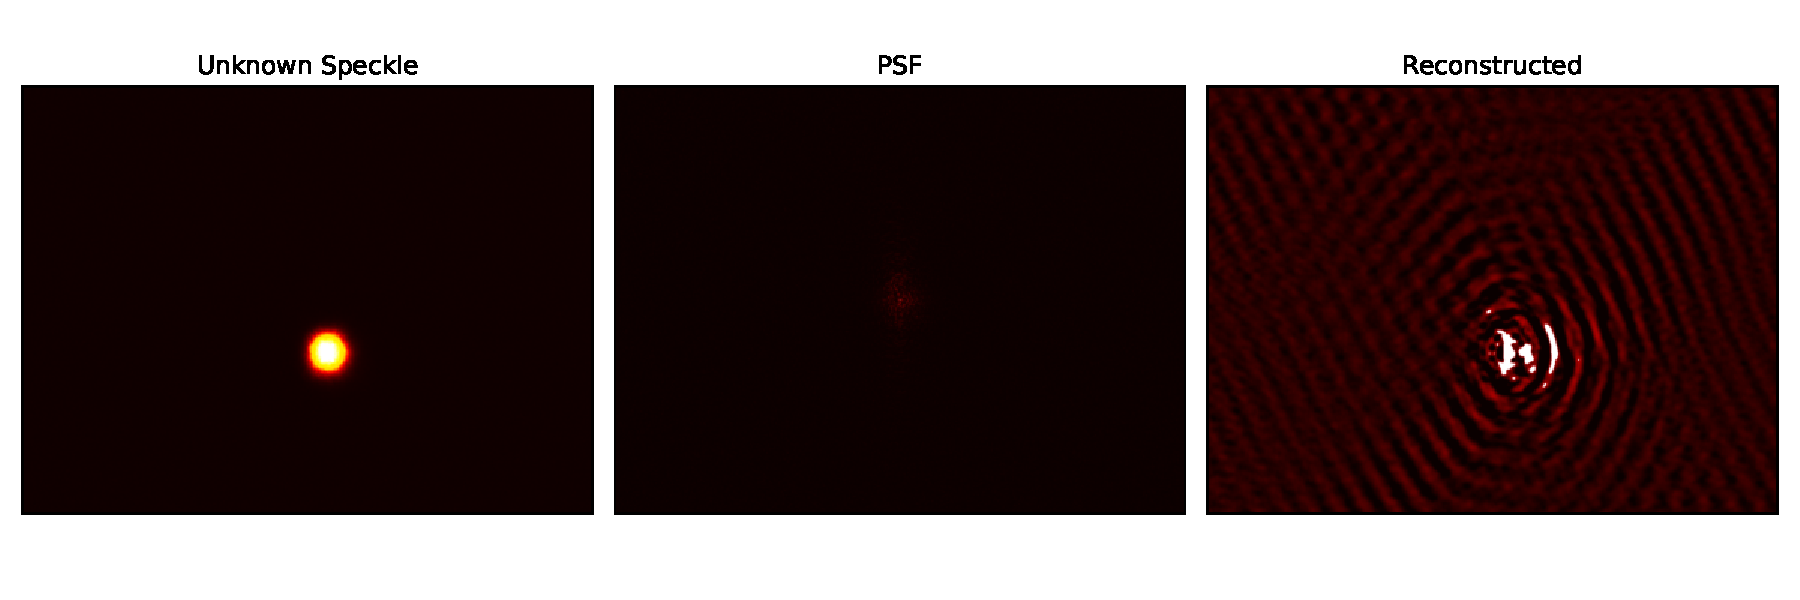
\includegraphics[width=0.8\linewidth]{实验二/工作距离的影响/工作距离50cm/图像对比图.pdf}
          \caption{工作距离50cm图像对比图}
      \end{figure}

      % 工作距离60cm
      \begin{figure}[H]
          \centering
          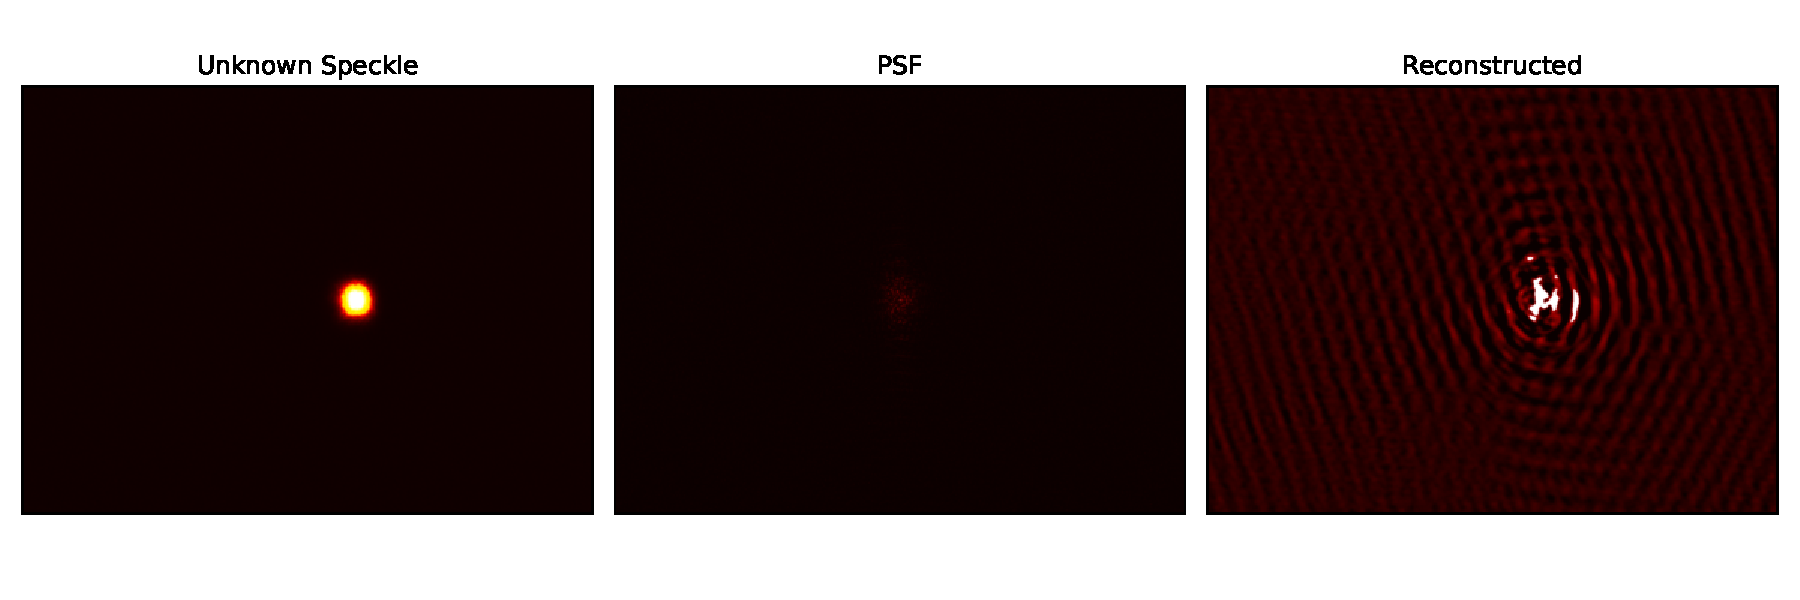
\includegraphics[width=0.8\linewidth]{实验二/工作距离的影响/工作距离60cm/图像对比图.pdf}
          \caption{工作距离60cm图像对比图}
      \end{figure}
      根据实验图像来看,均无明显的较好效果。分析原因后,我们发现主要是两个原因导致重建失败,一个是“图像过曝”,导致高频的信息缺失;一个是整个光路未对齐,导致出现像差,使得散斑所携带的信息被识别成了噪声。
      
      之后我们重新调整了光路,重新测量了这部分实验内容,见后。

    \item 第二次实验

      \begin{figure}[H]
          \centering
          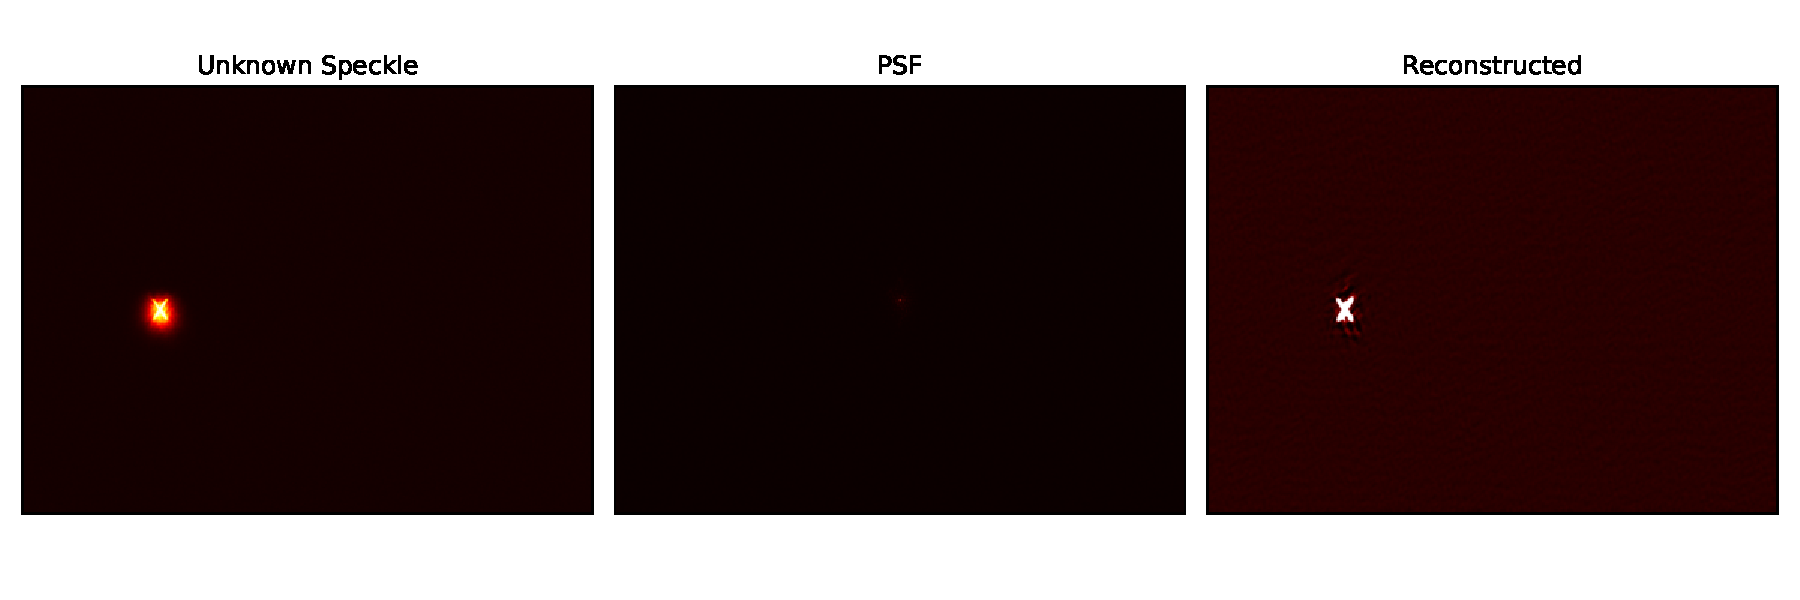
\includegraphics[width=0.8\linewidth]{二次实验/50cm_2/图像对比图.pdf}
          \caption{工作距离50cm图像对比图}
      \end{figure}

      \begin{figure}[H]
          \centering
          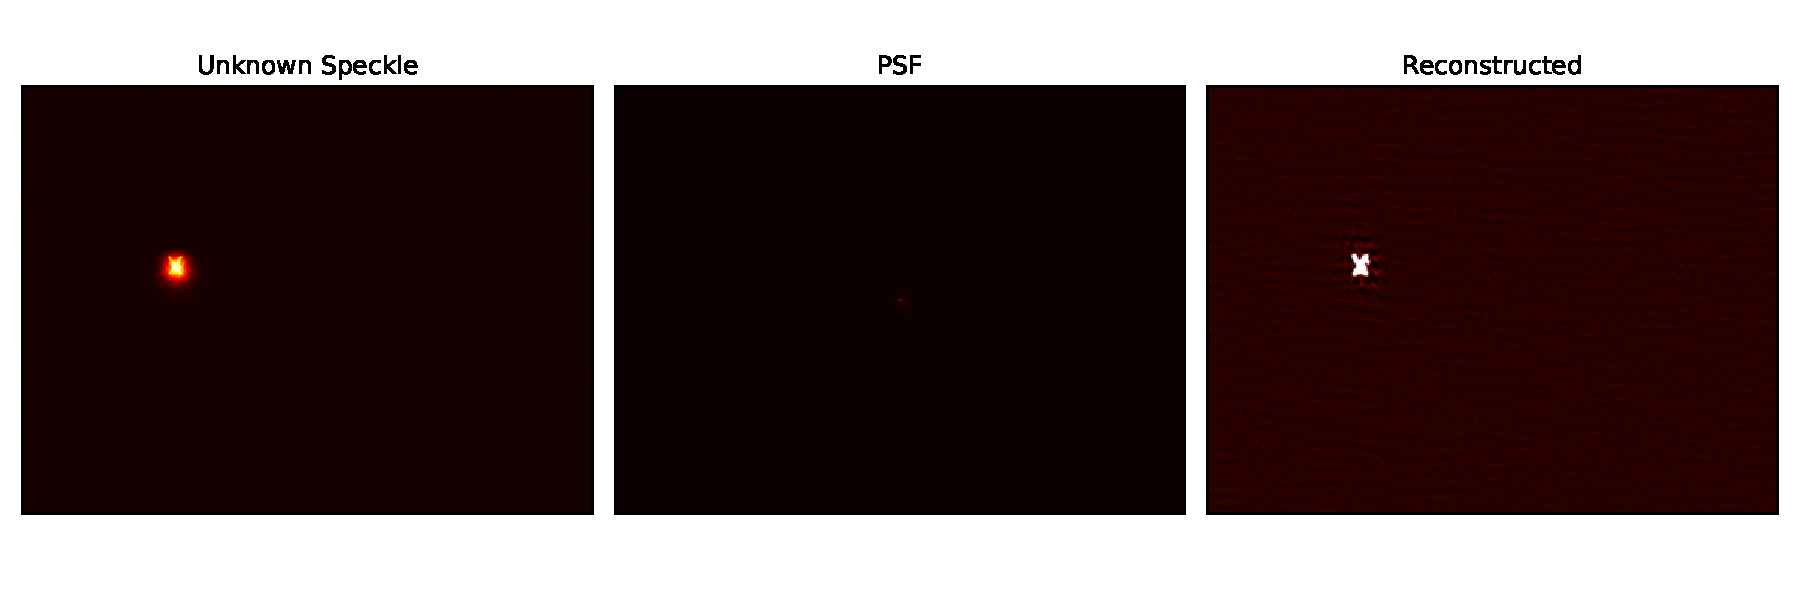
\includegraphics[width=0.8\linewidth]{二次实验/55cm_2/图像对比图.pdf}
          \caption{工作距离55cm图像对比图}
      \end{figure}
      \begin{figure}[H]
          \centering
          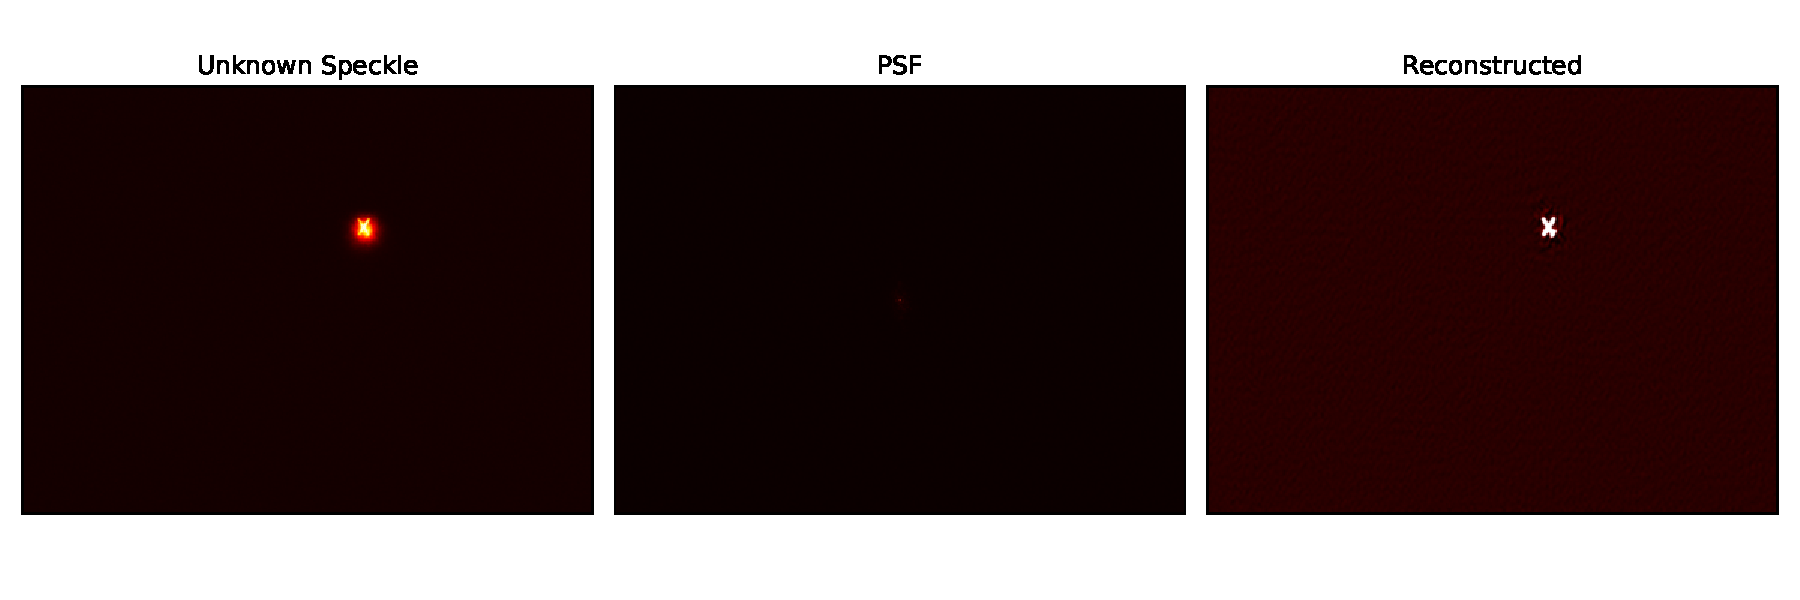
\includegraphics[width=0.8\linewidth]{二次实验/60cm_2/图像对比图.pdf}
          \caption{工作距离60cm图像对比图}
      \end{figure}
 
      % 观察可以发现,工作距离越长,成像效果变差了一点,但是具体来看,在这个实验条件下,可能的确影响不大。    
      理论上,工作距离决定了系统对散斑图的角度分辨能力和信噪比,从而显著影响图像重建效果。距离过短时,角度扰动引起的散斑位移不明显,难以利用记忆效应重建图像;而距离过长虽可放大角度响应,有利于记忆效应的利用,但信号衰减严重,噪声上升,系统更易受干扰。因此,应在角度灵敏度与信噪比之间取得平衡,选择适中的工作距离以获得最佳重建效果。

      由我们的实验结果可知,在我们的实验条件下,工作距离范围较大,在($L \in (50, 60)$cm)的范围内均能够重建图像。




    \end{itemize}
  




\subsubsection{不同散射片}
% ============ 不同散射片 ============
  % 0.5° 散射片
  \begin{figure}[H]
      \centering
      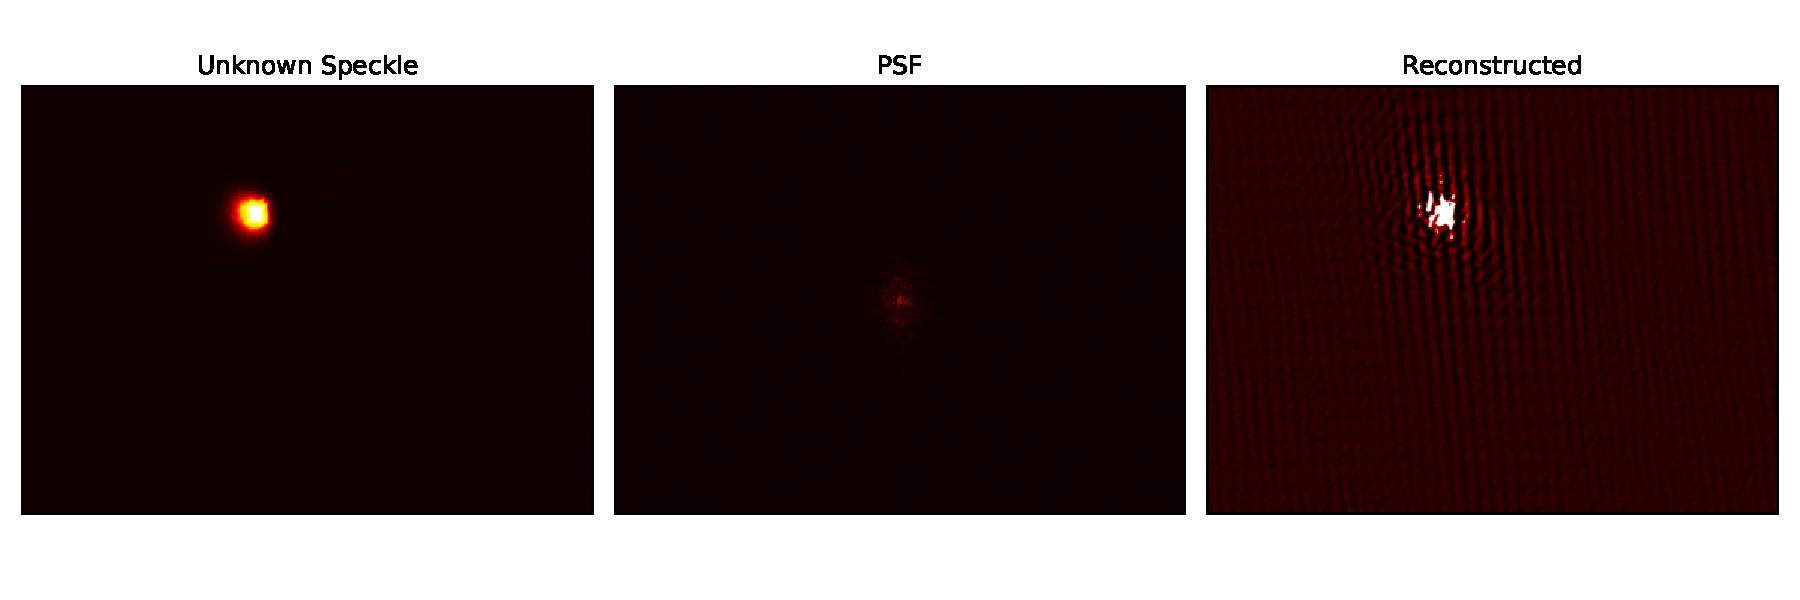
\includegraphics[width=0.8\linewidth]{实验二/不同散射片/0.5°/图像对比图.pdf}
      \caption{0.5°散射片图像对比图}
  \end{figure}

  % 5° 散射片
  \begin{figure}[H]
      \centering
      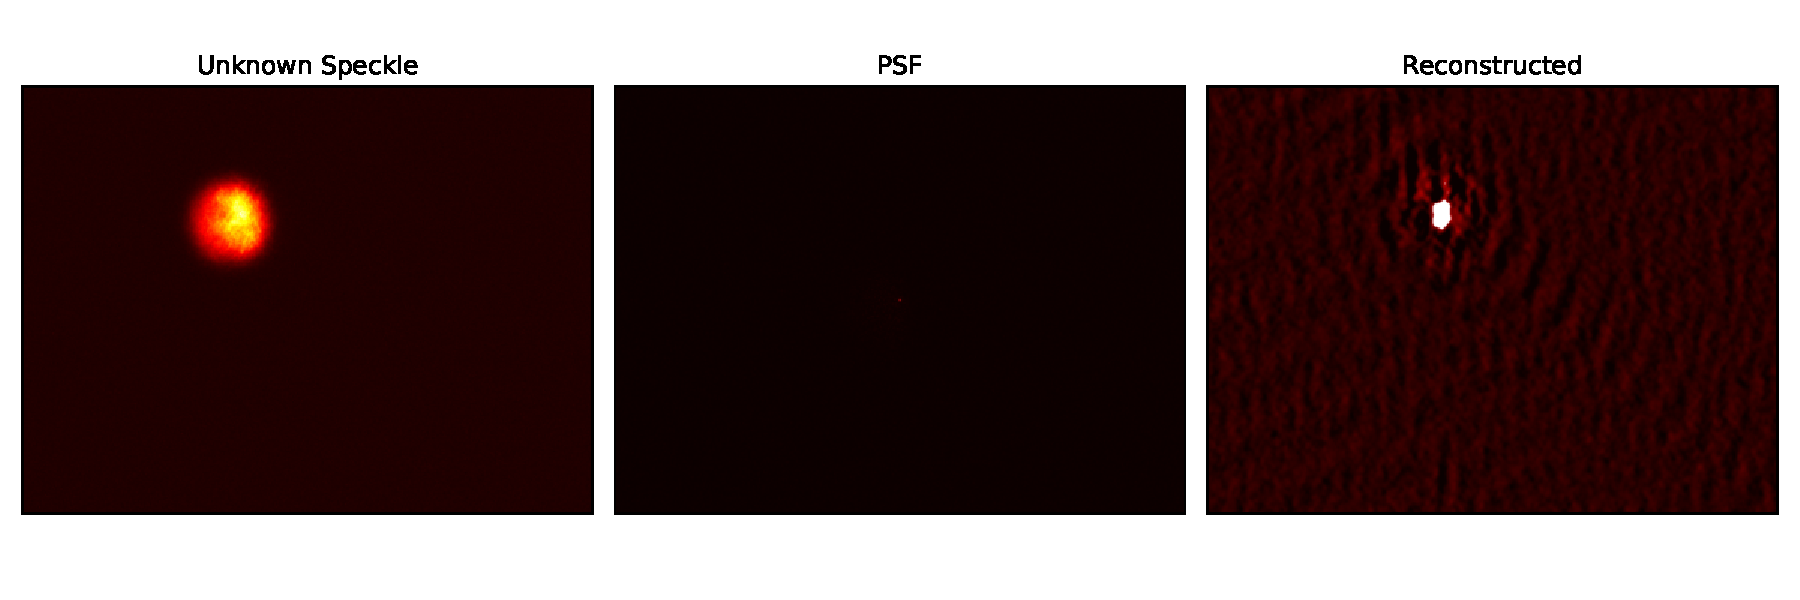
\includegraphics[width=0.8\linewidth]{实验二/不同散射片/5°/图像对比图.pdf}
      \caption{5°散射片图像对比图}
  \end{figure}

  % 10° 散射片
  \begin{figure}[H]
      \centering
      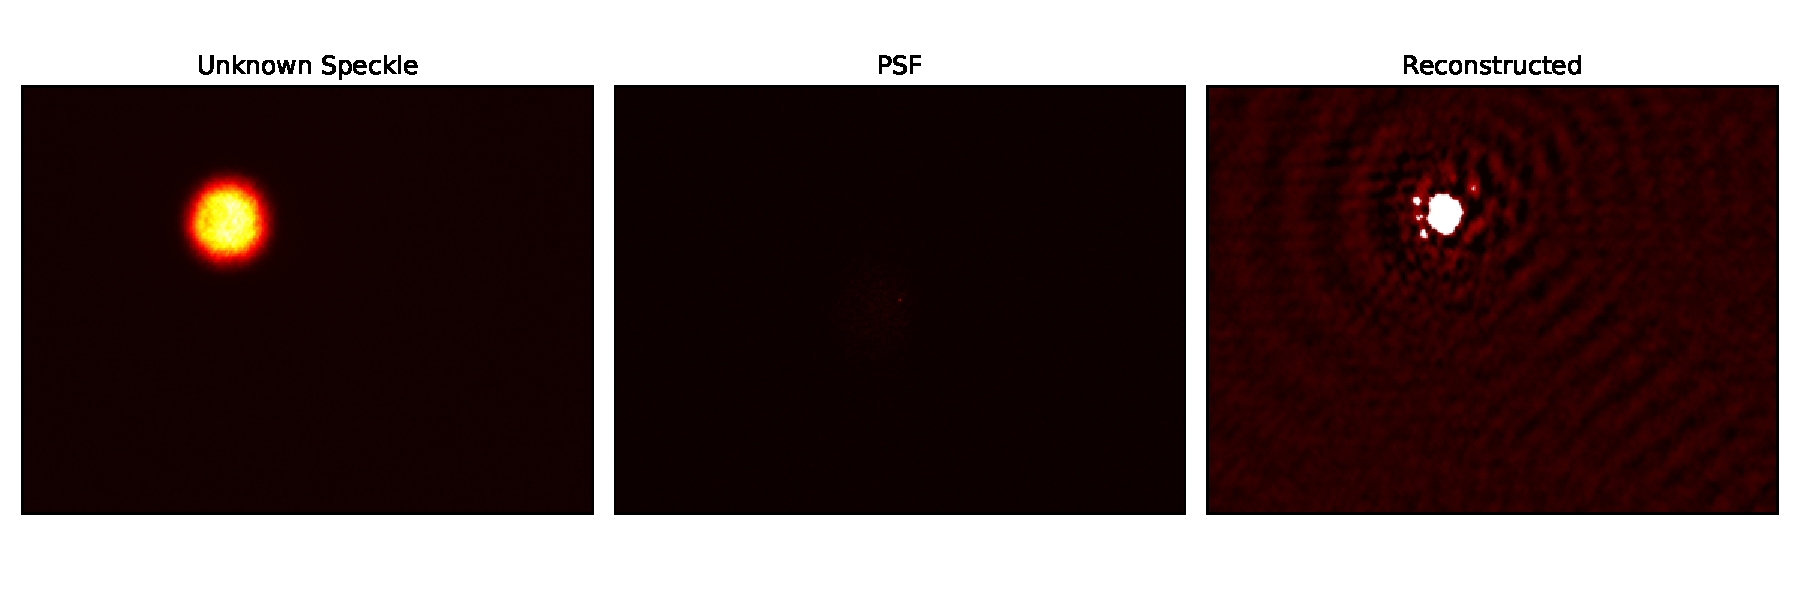
\includegraphics[width=0.8\linewidth]{实验二/不同散射片/10°/图像对比图.pdf}
      \caption{10°散射片图像对比图}
  \end{figure}

  % 同散射片,随着散射片角度的增大,成像效果越来越差。
  在本实验中,我们通过更换不同度数的散射片,探究不同条件对散射光成像的影响。

  可以看到,在实验一中,我们使用 1° 的散射片进行相关测量,能够成功重建图像;在此实验中,我们更换了 0.5°、5°、10° 的散射片,均不能成功重建图像。

  对于 5°、10° 两种散射片,其散射过强,入射光经过大量多次散射,路径混合,所以微小角度或位移改变不会导致出射场的规律性移动,而是完全重构,导致出射光场中不再保留可用于重建的信息;对于 0.5° 的散射片,我们认为其被过度使用导致其实际散射效果超过标称的 0.5°,导致重建失败。




\subsubsection{总结}

  本实验通过改变旋转角度、焦距、工作距离及散射片种类,分析了不同条件对散射光成像效果的影响。
  
  结果表明:轻微旋转散射片仍能保持较高的散斑相关性,图像可重建,体现了旋转记忆效应;适当焦距有助于平衡视场和角度分辨率,提升成像质量;合适的工作距离可增强角度扰动对散斑的响应,利于图像恢复;而散射角过大会破坏图像重建条件,1°散射片在保持足够散斑特征与空间相关性的同时,实现了较好的重建效果。



    
    % 附录(包含补充材料、个人签名、实验台整理情况、原始数据记录、实验附表、代码及参考文献)
    
\clearpage
\JMSection{附录}

\subsection{补充材料}

\begin{enumerate}
	\item 本实验报告内容由黄罗琳、戴鹏辉共同完成,小组成员分工明确,工作任务平均。
	\item 感谢两位老师在实验中详细为我们解答每一个问题,让我们能够按时完成实验,感谢您!
	\item 相关源文件(Latex)已上传Github,相关库包含实验报告内容,如需要查看可联系我进行查阅。
\end{enumerate}
\quad \large \textbf{感谢您对于此篇实验报告的阅读与批改,祝您工作顺利!}

\subsection{原始数据与桌面}
\begin{figure}[H]
    \centering
    \begin{minipage}{0.4\textwidth} % 设置第一个图片的宽度
        \centering
        \includegraphics[width=\linewidth]{app1.jpg}
        \caption{原始数据与签名}
        \label{}
    \end{minipage}%
    \hfill
    \begin{minipage}{0.4\textwidth} % 设置第二个图片的宽度
        \centering
        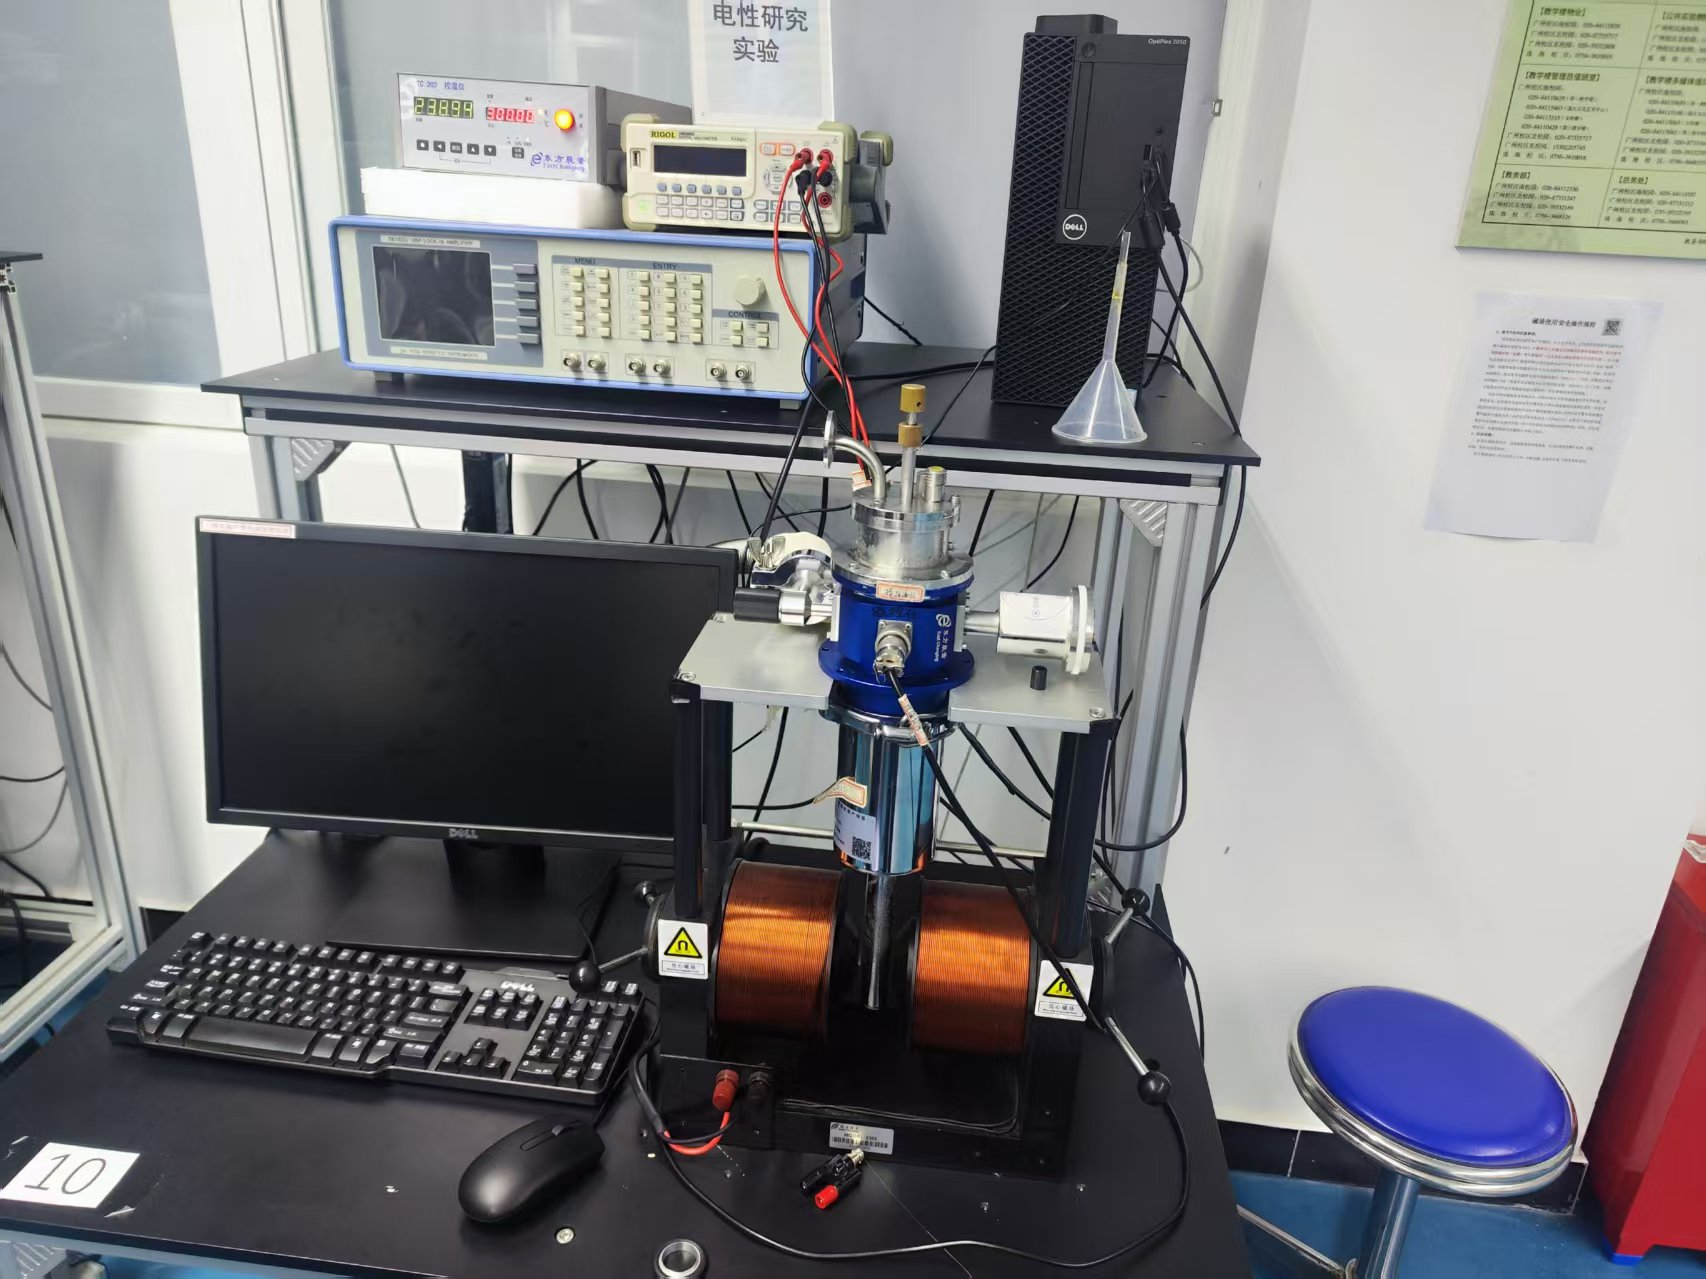
\includegraphics[width=\linewidth]{app2.jpg}
        \caption{整理后桌面}
        \label{}
    \end{minipage}
\end{figure}

\subsection{个人签名}
\begin{figure}[H]
    \centering
    \begin{minipage}{0.45\textwidth} % 第一个图片的宽度
        \centering
        \includegraphics[width=\linewidth]{签字.jpg}
        \caption{个人签名:黄罗琳}
        \label{}
    \end{minipage}%
    \hfill
    \begin{minipage}{0.45\textwidth} % 第二个图片的宽度
        \centering
        \includegraphics[width=\linewidth]{dph.jpg}
        \caption{个人签名:戴鹏辉}
        \label{}
    \end{minipage}
\end{figure}

\begin{figure}[htbp]
    \centering
    \begin{minipage}{0.7\textwidth} % 第三个图片的宽度
        \centering
        
\includegraphics[width=\linewidth]{name.png}
        \caption{个人签名:杨舒云}
        \label{fig:name}
    \end{minipage}
\end{figure}

\begin{figure}[H]
    \centering
    \begin{minipage}{0.45\textwidth} % 第四个图片的宽度
        \centering
        \includegraphics[width=\linewidth]{dhk.png}
        \caption{个人签名:丁侯凯}
        \label{}
    \end{minipage}
\end{figure}



    
\end{document}
